\documentclass[draft=false
              ,paper=a4
              ,twoside=false
              ,fontsize=11pt
              ,headsepline
              ,BCOR10mm
              ,DIV11
              ]{scrbook}
\usepackage[ngerman,english]{babel}
%% see http://www.tex.ac.uk/cgi-bin/texfaq2html?label=uselmfonts
\usepackage[T1]{fontenc}
\usepackage[utf8]{inputenc}
%\usepackage[latin1]{inputenc}
\usepackage{libertine}
\usepackage{pifont}
\usepackage{microtype}
\usepackage{textcomp}
\usepackage[german,refpage]{nomencl}
\usepackage{setspace}
\usepackage{makeidx}
\usepackage{listings}
\usepackage{natbib}
\usepackage[ngerman,colorlinks=true]{hyperref}
\usepackage{soul}
\usepackage{hawstyle}
\usepackage{lipsum} %% for sample text
\usepackage{tocbibind}
\usepackage{amsmath} 
\usepackage{amssymb}
\usepackage{hyperref}
\usepackage[section]{placeins}
\usepackage{grffile}

%% define some colors
\colorlet{BackgroundColor}{gray!20}
\colorlet{KeywordColor}{blue}
\colorlet{CommentColor}{black!60}
%% for tables
\colorlet{HeadColor}{gray!60}
\colorlet{Color1}{blue!10}
\colorlet{Color2}{white}

%% configure colors
\HAWifprinter{
  \colorlet{BackgroundColor}{gray!20}
  \colorlet{KeywordColor}{black}
  \colorlet{CommentColor}{gray}
  % for tables
  \colorlet{HeadColor}{gray!60}
  \colorlet{Color1}{gray!40}
  \colorlet{Color2}{white}
}{}
\lstset{%
  numbers=left,
  numberstyle=\tiny,
  stepnumber=1,
  numbersep=5pt,
  basicstyle=\ttfamily\small,
  keywordstyle=\color{KeywordColor}\bfseries,
  identifierstyle=\color{black},
  commentstyle=\color{CommentColor},
  backgroundcolor=\color{BackgroundColor},
  captionpos=b,
  fontadjust=true
}
\lstset{escapeinside={(*@}{@*)}, % used to enter latex code inside listings
        morekeywords={uint32_t, int32_t}
}
\ifpdfoutput{
  \hypersetup{bookmarksopen=false,bookmarksnumbered,linktocpage}
}{}

%% more fancy C++
\DeclareRobustCommand{\cxx}{C\raisebox{0.25ex}{{\scriptsize +\kern-0.25ex +}}}

\clubpenalty=10000
\widowpenalty=10000
\displaywidowpenalty=10000

% unknown hyphenations
\hyphenation{
}

%% recalculate text area
\typearea[current]{last}

\makeindex
\makenomenclature

\begin{document}
\selectlanguage{ngerman}

%%%%%
%% customize (see readme.pdf for supported values)
\HAWThesisProperties{Author={Andreas Müller, Claus Torben Haug, Jan Dennis Bartels, Marjan Bachtiari}
                    ,Title={MBC-Ping-Pong}
                    ,EnglishTitle={MBC-Ping-Pong}
                    ,ThesisType={Projektarbeit}
                    ,ExaminationType={Wahlpflichtfach}
                    ,DegreeProgramme={Bachelor of Science Angewandte Informatik}
                    ,ThesisExperts={Prof. Dr. Martin Becke}
                    ,ReleaseDate={\today}
                  }

%% title
\frontmatter

%% output title page
\maketitle

\onehalfspacing

%% add abstract pages
%% note: this is one command on multiple lines
\HAWAbstractPage
%% German abstract
{Ping-Pong, NodeJS, JavaScript, WebRTC}%
{In diesem Dokument wird das Projekt im MBC-Ping-Pong, das im Rahmen des Wahlpflichtfaches Modernebrowserkommunikation an der HAW-Hamburg erstellt wird, behandelt. Hierbei handelt es sich um eine Pong Clone welcher auf einem zentralen Bildschirm spielbar ist und mnittels WebRTC gesteuert wird. Es wird auf die Architektur, JavaScript, Frontend und Backend eingegangen. }
%% English abstract
{Ping-Pong, NodeJS, JavaScript, WebRTC}%
{This document is about the Project MBC-Ping-Pong, which is made for the elective course Modernebrowserkommunikation at HAW-Hamburg. Its about a Pong clone, played on a central screen nd controled via WebRTC. The architecture, JavaScript, frontend and backend are discussed. }

\newpage
\singlespacing

\tableofcontents
\newpage
%% enable if these lists should be shown on their own page
\listoftables
\listoffigures
%%\lstlistoflistings

%% main
\mainmatter
\onehalfspacing
%% write to the log/stdout
\typeout{===== File: chapter 1}
%% include chapter file (chapter1.tex)
%%\include{chapter1}

\chapter{Architektur}

\section{Arbeitsablauf zur Bearbeitung eines Issue}
Um eine erfolgreiche Zusammenarbeit zu gewährleisten, sind allgemein gültige Regeln nötig. Insbesondere wird festgelegt, wie die einzelnen Arbeitsschritte ablaufen sollten, um ein Issue zu bearbeiten. Zudem werden weiterhin die Zuständigkeiten geregelt. 

\subsection{Verwaltung der zu bearbeitenden Issues}
Die zu bearbeitenden Issues werden auf GitHub unter Issues (\href{https://github.com/Transport-Protocol/MBC-Ping-Pong/issues}{https://github.com/Transport-Protocol/MBC-Ping-Pong/issues}) gepflegt. Um den Verlauf eines Issues darzustellen wird das Kanbanboard von GitHub (\href{https://github.com/Transport-Protocol/MBC-Ping-Pong/projects}{https://github.com/Transport-Protocol/MBC-Ping-Pong/projects}) genutzt.

\subsection{Erstellen der zu bearbeitenden Issues}
Prinzipiell kann und darf jedes Projektmitglied zu jeder Zeit Issues erstellen. Gerade bei Bugs ist dies ein gewünschtes vorgehen. In der Regel sollten dies jedoch aus Gruppensitzungen hervorgehen und durch den Architekten ausformuliert werden.\newline
Ein Issue besteht aus drei Absätzen:
\begin{itemize}
	\item \textbf{Beschreibung} \newline
	In der Beschreibung wird allgemein auf den Kontext des Issues eingegangen.
	\item \textbf{Anforderung} \newline
	In Anforderung wird die Zielvision dargestellt.
	\item \textbf{Abnahmekriterien} \newline
	In Abnahmekriterien werden alle Punkte aufgeführt, die notwendig sind, um das Issue als erfolgreich bearbeitet anzusehen.
\end{itemize}

\subsection{Das Kanbanboard}
Das Kanbanboard ist in fünf Abschnitte eingeteilt: 
\begin{itemize}
	\item \textbf{Selected for Development} \newline
	Diese Spalte enthält alle Issues, die der Architekt zur Bearbeitung in nächster Zeit ausgewählt hat. Hier enthaltene Issues sind entweder durch den Architekten einem bestimmten Teammitglied zugeordnet. Diese sollten dann auch vorrangig bearbeitet werden. Oder (dies sollte der Normalfall sein) sie sind niemandem zugeordnet, dann kann sich jedes Teammitglied entscheiden, ob er das Issue bearbeitet. Gründe für das direkte zuweisen können unteranderem sein, dass es eine entsprechende vorhergehende Absprache gab, dass der Architekt das Issue speziell einem Bereich zugehörig sieht bzw. eine spezielle Paarung erreichen möchte, oder aber auch, weil ein Issue schon zu lange in "Selected for Development" verweilt. Hat sich ein Teammitglied für ein Issue entschieden, trägt er sich als Bearbeiter ein und zieht es in auf "In Development".
	\item \textbf{In Development} \newline
	In dieser Spalte verweilen alle Issues, an denen gerade entwickelt wird. Wenn die Entwicklung an einem Issue abgeschlossen ist, zieht der Bearbeiter das Issue weiter auf "Needs Review".
	\item \textbf{Needs Review} \newline
	Hier verweilen alle Issues, deren Entwicklung abgeschlossen ist, aber noch nicht geprüft wurde, ob die Abnahmebedingungen erfüllt sind. Normalerweise sollte die Abnahme durch den Architekten erfolgen. Issues, die der Architekt bearbeitet hat, muss das Review von einem anderen Teammitglied gemacht werden. Ein Issue bei dem das Review durchgeführt wird, wird in die Spalte "In Review" verschoben.
	\item \textbf{In Review} \newline
	Hier sind alle Issues enthalten, die sich gerade im Review befinden. Sind alle Abnahmekriterien erfüllt, und sind durch die Bearbeitung des Issue keine neuen Probleme/Fehler hinzugekommen, wird es in die Spalte "Done" verschoben und das Issue geschlossen. Ist dies nicht der Fall, wird ein Entsprechender Kommentar mit einer möglichst detaillierten Beschreibung des Problems an das Issue angehängt, und es wieder auf "In Development" geschoben. 
	\item \textbf{Done} \newline
	Diese Spalte enthält alle abgeschlossenen Issues.
\end{itemize}

\subsection{Git}
Hier sind die Verhaltensweisen für die Nutzung von Git aufgeführt. Alles hier nicht aufgeführte kann von jedem Teammitglied nach eigenen ermessen gehandhabt werden.
\begin{itemize}
	\item \textbf{Branches} \newline
	Für jedes Issue wird ein Branch erstellt, außer es handelt sich um reine Dokumentation (im Ordner Docu). Ein Branchname folgt folgendem Muster: "\#<IssueNummer> <KurzerName>". Dadurch lässt sich 
	\item \textbf{Commits} \newline
	Commits folgen folgendem Namensschema: "\#<IssueNummer> <Beschreibung>".
	\item \textbf{Push und Pull} \newline
	Es sollte möglichst häufig gepusht werden, um einen eventuellen Datenverlust zu vermeiden. Beim Pull sollte mit "--rebase" gearbeitet werden, um die Historie möglichst sauber zu halten.
	\item \textbf{Merge und Pullrequest} \newline
	Bevor ein Issue auf "Needs Review" geschoben wird, ist der Master in den Branch zu mergen und ein Pullrequest (\href{https://github.com/Transport-Protocol/MBC-Ping-Pong/pulls}{https://github.com/Transport-Protocol/MBC-Ping-Pong/pulls}) zu erstellen. Derjenige der das Issue reviewt hat, merget den Branch dann mithilfe des Pullrequests in den Master und löscht ihn.
\end{itemize}

\section{Meilensteine}
In diesem Abschnitt werden die Meilensteine festgelegt. Hierbei wird beschrieben, was wan erreicht sein sollte.
\subsection{Projekt Aufsetzen}
\begin{itemize}
	\item \textbf{Beschreibung}\newline
	Die Grundlegenden für die Entwicklung notwendigen anfangs Infrastrukturen sind aufgesetzt.
	\item \textbf{Kriterien}
	\begin{itemize}
		\item \textbf{NodeJS-Server aufsetzen} \newline
		Der NodeJS Server ist aufgesetzt und stellt eine statische Website zur Verfügung
		\item \textbf{Docker} \newline
		Eine einheitliche Umgebung wird durch Docker und Docker-Compose ermöglicht.
	\end{itemize}
	\item \textbf{Beendet:} 25.11.2016
\end{itemize}

\subsection{Prototyp (Technik)}
\begin{itemize}
	\item \textbf{Beschreibung}\newline
	Um die identifizierten technischen Risiken schnellst möglich in den Griff zu bekommen, werden diese möglichst früh bearbeitet. In dem Prototyp (Technik) soll gezeigt werden, das die kritische Technik funktioniert. Dies wird anhand von kleine losgelösten Beispielen, die aber nahe der Zielarchitektur sind gezeigt.
	\item \textbf{Kriterien}
	\begin{itemize}
		\item \textbf{Darstellung} \newline
		Es wird gezeigt, das im Webbrowser eine Flüssige Darstellung möglich ist.
		\item \textbf{Kollisionserkennung} \newline
		Es wird gezeigt, dass eine Kollisionserkennung erreichbar ist.
		\item \textbf{Kommunikation mittels WebRTC} \newline
		Architektur bedingt ist die Nutzung von WebRTC unumgänglich. Es ist zu zeigen, dass eine Verbindung von mehreren Handys zum Darstellungsmedium möglich ist.
		\item \textbf{Steuerung} \newline
		Die Steuerung soll über den Touchscreen geschehen. Es ist zu zeigen, dass es möglich ist, die Position des Fingers auf dem Touchscreen im Browser auszulesen. 
		\item \textbf{Größen der Handys/Tabletts} \newline
		Unterschiedliche Handys und Tabletts haben verschiedene Größen und Formen. Somit ist ein Konzept zu erarbeiten, welches diesem Problem bei der Steuerung gerecht wird.
	\end{itemize}
	\item \textbf{Beendet:} 16.12.2016
\end{itemize}

\subsection{Release 1.0 (Zwei Spieler)}
\begin{itemize}
	\item \textbf{Beschreibung}\newline
	In diesem ersten Release ist eine Basisversion des Spieles implementiert. Es können zwei Spieler gegeneinander Spielen, indem sie ihre Schläger mit den Handys steuern. Gleichzeitig ist diese Version die minimal Version und enthält alle "Must"-Features.
	\item \textbf{Kriterien}
	\begin{itemize}
		\item \textbf{Schläger} \newline
		Für jeden Spieler existiert ein Schläger, der mit dem Handy Steuer
		\item \textbf{Ball} \newline
		Es gibt ein Ball, der sich über das Spielfeld bewegt. Kollidiert er mit einem Schläger oder der Wand, an der sich kein Schläger befindet, prallt er davon ab. Es gilt hierbei, dass der Einfallwinkel dem Ausfallwinkel entspricht. Zudem beschleunigt der Ball, wenn er mit einem Schläger kollidiert. Wenn der Ball mit der Wand hinter einem Schläger kollidiert, wir er in die Ausgangsposition versetzt und erhält die Ausgangsgeschwindigkeit.
		\item \textbf{Punkte} \newline
		Immer wenn der Ball mit der Wand hinter einem Schläger kollidiert, erhält der andere Spieler einen Punkt.
		\item \textbf{Spielende} \newline
		Das Spiel endet automatisch nach X Spielen (wobei gilt: $X \in  \mathbb{N} \land X \mod 2 = 1$ ). \textit{Das genaue X ist noch zu definieren.}
	\end{itemize}
	\item \textbf{Beendet:} 13.01.2017
\end{itemize}

\subsection{Release 1.X (Diverse Features)}
\begin{itemize}
	\item \textbf{Beschreibung}\newline
	Basierend auf der Version 1.0 wird das Spiel weiterentwickelt. Jedoch sind alle Features die hier bearbeitet werden können "Can"-Features. Daher kann es sein, dass das Release 1.X äquivalent zu dem Release 1.0 ist. Zudem sind alle hier genannten möglichen Features noch nicht näher spezifiziert und auf ihre Machbarkeit geprüft. Es gilt jedoch, dass je Umgesetztes Feature die Versionsnummer im Minorbereich um Eins steigt.
	\item \textbf{mögliche Kriterien}
	\begin{itemize}
		\item \textbf{N Spieler} \newline
		Mehr als 2 Spieler
		\item \textbf{Zusätzliche Hindernisse} \newline
		Auf dem Spielfeld sind zusätzliche Hindernisse.
		\item \textbf{Highscore-Liste} \newline
		Es wird eine Highscore-Liste geführt und angezeigt.
		\item \textbf{TBD} \newline
		To be discussed.
	\end{itemize}
	\item \textbf{Beendet:} 24.02.2017
\end{itemize}

\section{Highlevel View}
In diesem Abschnitt wird die Grob-/Gesamtarchitektur betrachtet. Hierbei wird nicht nur auf wesentliche Schnittstellen und Komponenten eingegangen. Zur engeren Auswahl standen zwei mögliche Ansätze. Es werden beide betrachtet, und erläutert warum der Ansatz 2 umgesetzt werden wird.
\subsection{Ansatz 1}
\begin{figure}[ht]
	\centering
	\includegraphics[width=0.9\textwidth]{architecture/highLevelAnsatz1.png}
	\caption{Highlevel Ansatz 1}
	\label{fig1}
\end{figure}

\subsection{Ansatz 2}
\begin{figure}[ht]
	\centering
	\includegraphics[width=0.9\textwidth]{architecture/highLevelAnsatz2.png}
	\caption{Highlevel Ansatz 2}
	\label{fig1}
\end{figure}







\chapter{JavaScript}

\chapter{Backend}


\section{Benennungen}
Folgend einige Begriffe, die häufig verwendet werden.
\begin{description}
\item[Multi-Peer]
Ein Multi-Peer ist ein Peer, welcher gleichzeitig Verbindungen zu mehreren anderen Peers pflegt.

\item[Single-Peer]
Ein Single-Peer ist ein Peer, welcher nur eine Verbindung zu einem anderen Peer pflegt.

\item[ControlPeer]
Der ControlPeer ist in diesem Projekt ein Peer, welcher Steuereingaben von dem Spieler annimmt und an den OutputClient sendet.

\item[OutputClient]
Der OutputClient ist in diesem Projekt ein Peer, welcher die Steuerangaben von den ControlPeer zugesendet bekommst und diese auswertet.
\end{description}



\section{Kommunikation}

\subsection{Zeitkritische Informationen}
Als zeitkritisch werden Informationen eingestuft, sofern sie die direkten 
Eingaben eines Peers, hier der ControlClients, und eventuelles Feedback eines anderes Peers, hier des OutputClient, betreffen. 
Da es sich bei diesem Projekt um ein Reaktionsspiel handelt, müssen diese Daten zeitnah von Sender 
zu Empfänger gelangen. Solch eine Relation ist nur über eine Peer-to-Peer 
Verbindung unter Verwendung von UDP zu realisieren.



\subsection{Möglichkeit 1: Predefined Packages 'rtc.io'}
Der NodeJS Server wird als Verbindungsserver für die Etablierung einer 
Peer-to-Peer Verbindung zwischen ControlClients und OutputClient genutzt. Als 
Technik wird konkret WebRTC eingesetzt. Auf dem NodeJS-Server wird das Package 
"rtc-switchboard" eingesetzt, welches eine Grundlage für einen  
Signalisierungsserver ist. Die Clients nutzen "rtc-quickconnect" um neues 
Channels anzufordern und eine Peer-to-Peer Verbindung zu etablieren.

\subsubsection{Vorteile}
\begin{itemize}
\item
Leichtere Implementierung, da alle Ebenen der Kommunikation bereits abgedeckt 
wurden und nur noch semantisch auf Informationen eingegangen werden muss.
\end{itemize}

\subsubsection{Nachteile}
\begin{itemize}
\item
Durch Generalisierung ein deutlicher Overhead.

\item
Status ist offiziell noch 'unstable'.
\end{itemize}



\subsection{Möglichkeit 2: Abstrakte WebRTC implementation 'WebRTC'}
Wie auch bei Möglichkeit 1 wird der NodeJS-Server als Verbindungsserver genutzt. 
Jedoch muss auf Client-Seite, also für OutputClient und ControlClient, eine 
eigene Signalling Implementation stattfinden. Es wird eine viel abtraktere 
Schicht genutzt.

\subsubsection{Vorteile}
\begin{itemize}
\item
Da die genutzen Packages nur eine Grundlage bilden, ist eine spezialisierte 
Implementierung möglich.
\end{itemize}

\subsubsection{Nachteile}
\begin{itemize}
\item
Implementierungsaufwand deutlich höher.

\item
Spezialisierung für dieses Projekt eventuell nicht nötig.

\item
Status ist offiziell noch 'unstable'.
\end{itemize}



\subsection{Möglichkeit 3: Socket.io-P2P}
Das Package Socket.io bietet auch selber eine Peer-to-Peer lösung auf WebRTC 
Basis. Hierbei wird eine Spezielle Art eines Sockets genutzt, welche wie ein 
normaler WebSocket agiert, bis ein Upgrade durchgeführt wird und die Clients nun 
direkt miteinander Kommunizieren.

\subsubsection{Vorteile}
\begin{itemize}
\item
Das Signalling und die P2P Kommunikation können mit einem Package geregelt 
werden.

\item
Variabel kann die Kommunikation über den Server, oder P2P ablaufen.

\item
Signalling events werden von Client-Server Kommunikation direkt zu P2P 
übernommen.
\end{itemize}

\subsubsection{Nachteile}
\begin{itemize}
\item
Wenig Einfluss auf die Upgrade-Mechanismen.

\item
Teils sehr instabil.
\end{itemize}



\subsection{Möglichkeit 4: Eigenes Kommunikationsmodul}
Aus Basis der WebRTC Standartimplementierung von den Browsern, kann eine eigene Schicht entwickelt werden, welche den Kommunikatinsaufbau (das Signalling) und die Kommunikationsabläufe regelt. 
Dies müsste auf einer generischen Basis geschehen um allen Anforderungen des Programmes gerecht zu werden.

\subsubsection{Vorteile}
\begin{itemize}
\item
Volle Kontrolle über Signalling und Verwaltungsabläufe der Verbindungen.

\item
Möglichkeit für schnelle Anpassungen.

\item
Unabhängigkeit gegenüber anderen Entwicklern.
\end{itemize}

\subsubsection{Nachteile}
\begin{itemize}
\item
Größter Implementierungsaufwand.

\item
Risikoabschätzung nur schwer möglich.

\item
Basis-Implementationen verschieden je Browser (gleiches Problem wie bei den anderen Implementationen: rtc.io, wocket.io-P2P, etc.)
\end{itemize}



\subsection{Statusinformationen}
Für den Austausch von Statusinformationen und Signalen zwischen Peer und Server werden WebSockets genutzt.
Für den Austausch von Statusinformationen zwischen Peers wird WebRTC genutzt.
Für den Austausch von Signalen zwischen Peers werden WebSockets genutzt, wobei der Server der Verbindungs-Knotenpunkt zwischen den Peers ist.



\subsection{Fazit nach Test}
Nach und auch schon während der Entwicklung des Prototypen hat sich 
rausgestellt, dass Socket.io-P2P in der Implementierung viele Fehler aufweist.
Gleiches gilt für rtc.io.
Eine teilweise Abänderung der Module (workarounds) führt näher an das gewünschte Ergebnis, 
verursacht aber intern wieder mehr Fehler und sorgt für eine inkonsistente Modulversion.



\subsection{Entscheidung}
Die eigene Implementation auf Basis des WebRTC bietet die meisten Möglichkeiten, birgt jedoch auch die meisten Risiken. 
RTC.io bietet eine Implementation die sehr gut für Prototypen geeignet ist, aber neben dem zeitunkritischen Signalling eine eigene Einheit bietet, welche eine Generalisierung des WebRTC darstellt und somit viel Overhead besitzt. 
Die P2P-Imeplementierung von Socket.io steht von der Implementierungs-Komplexität in der Mitte. 
Es bietet viele bereits bekannte Mechanismen des Client-Server Signalling über Events, welche mit einem Upgrade nun auch von Client zu Client funktionieren. 
Dagegen spricht jedoch die instabilität der P2P-Implementation von Socket.io. \\ \\

Eine eigene Implementation eines Modules auf Basis der von den Browsern gegebenen WebRTC-Schnittstelle ist die Wahl. 
Sie bietet die größtmögliche Flexibilität im Bezug auf Veränderbarkeit und Anpassung im laufenden Entwicklungszyklus. 
Als Risiko ist besonders der große Aufwand anzusehen.



\section{Eigenes Modul Kommunikation}

\subsection{Anforderungen an das eigene Modul für WebRTC}
\begin{itemize}
\item 
Es muss möglich sein, unsere ControlPeers nur mit dem DisplayPeer zu verbinden, 
nicht aber untereinander (Sterntopologie, wobei der DisplayPeer der Knoten ist).

\item
Der DisplayPeer muss zu jedem ihm zugeordneten ControlPeer verbunden sein.

\item
Es Muss auf Serverseite eine Raumlogik existieren, um die Peers zuordnen zu 
können.

\item
Das Signalling muss weiterhin über den Server stattfinden.
\end{itemize}



\subsection{Zuweisungslogik Server}
Der Server hat bezüglich der Zuweisungen für Verbindungen die Aufgabe alle 
Clients zu gruppieren. Dies soll ähnlich wie bei Socket.io über eine Raumlogik 
geschehen. Es existieren Räume, in welche die WebSockets auf dem Server (je Client 
also einer) eingeordnet werden.


Hierbei unterscheiden sich die Clients in ihrem Kommunikationsmodus:
\begin{description}
\item[Single]
Ein Client mit dem ''Single'' Modus pflegt nur eine direkte WebRTC Verbindung.

\item[Multi]
Ein Client mit dem ''Multi'' Modus pflegt mehrere direkte WebRTC Vebindungen 
gleichzeitig und agiert zwischen den ganzen Peers als "Host".
\end{description}

\begin{figure}[htH]
\centering
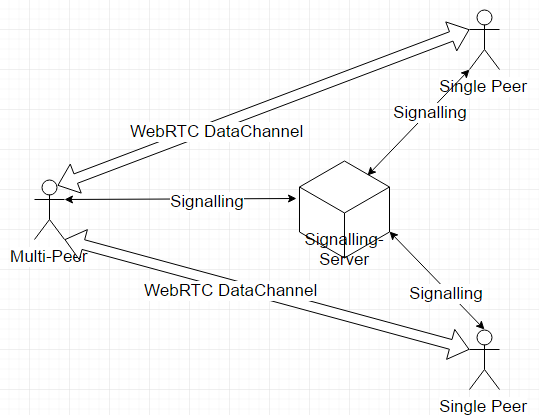
\includegraphics[width=0.9\textwidth]{backend/ConnectionBetweenPeers.PNG}
\caption{Verbindungsnetz}
\label{backfig1}
\end{figure}

In Abbildung \ref{backfig1} ist zu sehen, wie ein "Multi-Peer" mit mehreren 
"Single-Peer" gleichzeitig über WebRTC (konkret den DataChannel) kommuniziert, 
jeder einzelne "Single-Peer" aber nur mit dem einen "Multi-Peer". Zu sehen ist 
außerdem, dass das Signalling weiterhin für alle Peers über den 
Signalling-Server stattfindet, welcher hier auch gleichzeitig der WebServer ist.



\subsection{Zuweisungslogik Client (Single)}
Von nun an wird der Client der den Single Modus nutzt als "Single-Peer" 
bezeichnet.

Der Single-Peer pflegt nur eine WebRTC Verbindung, somit muss keine 
Zuweisungslogik geschehen.



\subsection{Zuweisungslogik Client (Multi)}
Von nun an wird der Client der den Multi Modus nutzt als "Multi-Peer" 
bezeichnet.


Der Multi-Peer pflegt mehrere WebRTC Verbindungen zu verschiedenen Single-Peers. 
Identifiziert werden die einzelnen Single-Peers über ein vom Server beim 
Signalling gesetztes Attribut in den Signalling Nachrichten: "from". Über dieses 
Attribut weiß der Multi-Peer von wem diese Signalling-Message kommt und kann so 
alle ankommenden Informationen diesem Single-Peer zuordnen. Somit wird unter dem 
Alias des Single-Peer ein eigenes "webRTCConnection"-Objekt verwaltet/abgelegt.
Verwendet wird hierzu ein "Assoziativer" Array, näheres in \ref{associativearray}.



\subsection{Identifizierung der Peers}
Die Peers selber erhalten in allen Signalling-Messages ein Attribut, über 
welches sie den Ursprung ermitteln können, um so Signale Peers zuordnen zu 
können. Diese \"ID'' wird vom Server vergeben und entspricht einfach nur der 
Socket ID welche die einzelnen Clients in Verbindung zum Server haben.
Da nur der Server diese ID vergibt ist diese auch eindeutig.



\section{Signalling Ablauf}
Der Ablauf ist bei den Single-Peers, sowie bei den Multi-Peers nahezu gleich.



\subsection{Anmeldung beim Server}
\begin{description}
\item[Multi-Peer]
Der Multi-Peer meldet sich beim Server mit der Bitte einen Raum zu erstellen. 
Sollte dieser Raum schon existieren ist dies ein Fehler, da in jedem Raum nur 
ein Multi-Peer existieren darf. Sollte der Raum noch nicht existieren, wird er 
erstellt und der Multi-Peer diesem zugewiesen.

\item[Single-Peer]
Der Single-Peer meldet sich beim Server mit der Bitte einen Raum zu betreten. 
Sollte dieser Raum noch nicht existieren ist dies ein Fehler, da ein Raum in 
diesem Projekt ein Spiel darstellt, ein Single-Peer (Control-Peer) aber nur 
einem bestehenden Spiel beitreten kann. Sollte der Raum bereits existieren und 
alle weiteren Spielablaufrelevanten Informationen stimmen (das Spiel darf zum 
Beispiel noch nicht angefangen haben), so tritt der Single-Peer diesem Raum bei. 
Direkt nach dem Beitreten eines Raumes, wird ein Signal an den Server gesendet, 
dass wir da sind.

\item[Server]
Sobald ein Raum existiert und ein Multi-Peer diesem zugewiesen ist, sendet jeder 
neu dazukommende Single-Peer ein Signal an den Server, dass er da ist. Dieses 
Signal wird nur an den Multi-Peer weitergeleitet.
\end{description}



\subsection{Erstes Signal}
\begin{description}
\item[Multi-Peer]
Jedes mal, wenn der Multi-Peer ein neues erstes Signal eines Single-Peers über 
den Server erhält ("hereandready"), ermittelt er seine ICE-Candidates (je nach Browser kann dieses Vorhaben eine erneute Ermittlung der Candidates, oder ein Verwenden der bereits vorher ermittelten veranlassen) und sendet 
diese an den Signalisierenden Single-Peer.
\end{description}



\subsection{ICE Candidates}
\begin{description}
\item[Multi-Peer]
Erhält ein Multi-Peer einen ICE-Candidate wird dieser der Passenden Verbindung 
hinzugefügt und löst das ''negotiationneeded''-Event aus, welches ein neues Offer 
in Form von SDP Signalisiert.

\item[Single-Peer]
Erhält ein Single-Peer einen ICE-Candidate wird dieser der akutellen 
webRTCCOnnection hinzugefügt und löst das "negotationneeded"-Event, welches ein 
neues Offer in Form von SDP Signalisiert.
\end{description}



\subsection{Aufbau über SDP}
\begin{description}
\item[Multi-Peer]
Erhält der Multi-Peer ein Offer in Form von SDP erwiedert er dieses mit einer 
Answer auch in Form von SDP und fügt die "remoteDescription" dieser 
WebRTCConnection auf Basis der Offer hinzu. Sofern dieser Vorgang Erfolg hatte 
ist eine direkte Verbindung zwischen Multi-Peer und Single-Peer entstanden.

\item[Single-Peer]
Erhält der Multi-Peer ein Offer in Form von SDP erwiedert er dieses mit einer 
Answer auch in Form von SDP und fügt die "remoteDescription" dieser 
WebRTCConnection auf Basis der Offer hinzu. Sofern dieser Vorgang erfolg hatte 
ist eine direkte Verbindung zwischen Multi-Peer und Single-Peer entstanden.
\end{description}



\subsubsection{Kommunikationskanal}
Da es sich um einfache Steuerungsdaten handelt verwenden beide Modi der Peers 
einen simplen DataChannel.



\section{Eigenes Modul: Aufbau}
\subsection{Eigenes Modul: Schnittstelle}
\begin{figure}[htH]
\centering
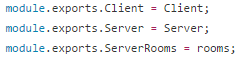
\includegraphics[width=0.9\textwidth]{backend/ModulExports.PNG}
\caption{Modul Exporte}
\label{backfig2}
\end{figure}

\begin{description}
\item[Modul.Client]
Unter Modul.Client ist eine Klassenorientierte Repräsentation des Clients zu 
finden. Es ist ein Object dieses Typs zu erzeugen.

\item[Modul.Server]
Unter Modul.Server ist eine Repräsentation des Servers zu finden. Für jeden auf 
dem Server neu Verbundenen Client muss eine neue (anonyme möglich) Instanz dieses Typs 
erstellt und dabei der WebSocket (socket.io), der mit dem Client verbunden, ist übergeben werden.

\item[Modul.ServerRooms]
Unter Modul.ServerRooms ist eine Simple Liste der derzeitigen Räume auf dem 
Server, inklusive der darin befindlichen Clients zu sehen. Diese Informationen 
sind jedoch nur auf Serverseite bei Verwendung des Modul.Server einsichtlich, 
bzw. werden nur unter Verwendung von Modul.Server aktualisiert.
\end{description}



\subsection{Eigenes Modul: Abhängigkeiten}
Das Modul ist derzeit direkt von Socket.io abhängig, von welchem es die 
WebSockets für das Signalisierungen über den Signalling-Server nutzt.



\subsection{Eigenes Modul: Struktur}
Das Modul implementiert zwei Teile. Erstens die Client-Seite. Zweitens die 
Server-Seite.



\subsubsection{Client Aufgaben}
Die Client-Implementation ist für das Frontend gedacht und nutzt alle WebRTC 
Standarts der Browserimplementationen (Mozilla, webkit und Microsoft überlagert). 
Es handelt alle Faktoren von Initiierung der Kommunikation, bis Durchführung dieser ab.



\subsubsection{Server Aufgaben}
Die Server-Implementation kümmert sich auf Server-Seite um die Einhaltung von 
Kommunikations-Standarts, die Zuweisung von Signalen und die Gruppierung vieler 
Peers.



\section{Eigenes Modul: Generischer Ansatz}

\subsection{Generische Anforderung}
Als Anforderung gilt, dass die Implementierung des Moduls von unserer Nutzung für das Ping-Pong Projekt entkoppelt ist. 
Dies ist als gegeben anzusehen, wenn die Implementation keine Hinweise auf dieses Projekt hinterlässt und Möglichkeiten zu Umsetzung anderer beliebiger Projekte bietet, ohne Anpassungen vornehmen zu müssen.



\subsection{Generische Umsetzung}
Im folgenden wird die allgemeine generische Umsetzung am Beispiel der Callbacks und Topologien gezeigt.



\subsubsection{Generische Umsetzung: Allgemein}
Im allgemeinen gibt es zwei Klassen von Peers, die ein Client nutzen kann.

\begin{quote}
  \begin{description}
  \item[Single-Peer]
  Ein Client der den Modus ''Single-Peer'' nutzt gibt damit an, dass er maximal eine direkte Verbindung zu einem anderen Peer pflegen möchte.

  \item[Multi-Peer]
  Ein Client der den Modus ''Multi-Peer'' nutzt gibt damit an, dass er eine oder mehr direkte Verbindungen zu Peers pflegen möchte.
  \end{description}
\end{quote}

Aus Kombinationen dieser Modi lassen sich verschiedene Topologien bilden. Näheres unter \ref{generictopology}.



\subsubsection{Generische Umsetzung: Callbacks}
Um jeden Nutzer dieses Moduls selbst die Verarbeitung von Ereignissen zu ermöglichen, ist die Möglichkeit gegeben, dass der Nutzer Callback-Funktionen hinterlegt, die bei gewissen autretenden Ereignissen ausgerufen werden.
Diese Ereignisse umfassen z.B:

\begin{quote}
  \begin{description}
  \item[Neue Verbindung]
  Eine neue Verbindung zu einem Peer wurde erfolgreich hergestellt.

  \item[Verbindungsverlust zu Peer]
  Eine bestehende Verbindung zu einem Peer wurde verloren.

  \item[Neue Nachricht]
  Es kam eine neue Nachricht über den DataChannel eines Peers an.
  \end{description}
\end{quote}

Weiteres zu der direkten Verwendung der Callback-Functionen unter \ref{callbacks}.



\subsubsection{Generische Umsetzung: Topologien} \label{generictopology}
Es lassen sich durch die Verwendung der zwei Modi verschiedene Topologien bilden.


\begin{quote}
  \begin{description}
  \item[one-to-one]
  Keine konkrete Topologie, aber für direkte Peer-to-Peer Verbindungen oft die gängiste Art. Beide Peers sind "Single-Peer" und pflegen jeweils nur die Verbindung zu dem anderen. 
  Siehe Abbildung \ref{backfig3}.
  \begin{figure}[htH]
  \centering
  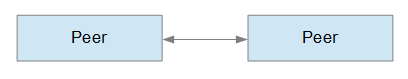
\includegraphics[width=0.9\textwidth]{backend/Topologie_1v1.PNG}
  \caption{Topologie one-to-one}
  \label{backfig3}
  \end{figure}

  \item[Stern]
  Einer der Peers agiert als Host für die anderen. Dieser Host-Peer ist der Mittelpunkt des Sternes und nutzt den Modus "Multi-Peer". Alle anderen Peers nutzen den Modus "Single-Peer" und pflegen nur die Verbindung zum Mittelpunkt (dem Host).
  Siehe Abbildung \ref{backfig4}.
  \begin{figure}[htH]
  \centering
  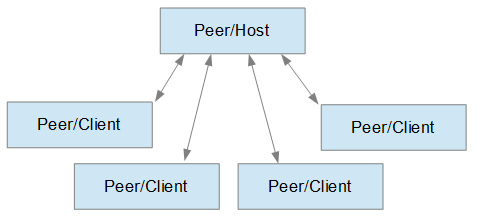
\includegraphics[width=0.9\textwidth]{backend/Topologie_4v1.PNG}
  \caption{Topologie Stern}
  \label{backfig4}
  \end{figure}

  \item[Vollvermascht]
  Alle Peers nutzen den Modus "Multi-Peer" und pflegen zu jedem anderen Peer eine direkte Verbindung.
  Siehe Abbildung \ref{backfig5}.
  \begin{figure}[htH]
  \centering
  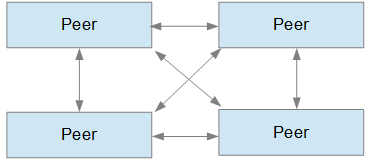
\includegraphics[width=0.9\textwidth]{backend/Topologie_ava.PNG}
  \caption{Topologie Vollvermascht}
  \label{backfig5}
  \end{figure}
  \end{description}
\end{quote}


\section{Eigenes Modul: Verwendung}

\subsection{Verwendung des Client}

\subsubsection{Abhängigkeiten}
\begin{figure}[htH]
\centering
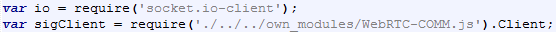
\includegraphics[width=0.9\textwidth]{backend/Modul_UserClientDependencies.PNG}
\caption{Dependencies Verwendung Client}
\label{backfig10}
\end{figure}
In Abbildung \ref{backfig10} sind die Clientseitigen Abhängigkeiten für das Modul zu sehen.
Die Client-Implementation von socket.io ''socket.io-client'' wird für das Signalling benötigt.
Zur Nutzung des Moduls muss dieses außerdem "required" werden. Hierzu wird der Pfad zu dem Modul als Parameter an das require übergeben und der Client Export genutzt.



\subsubsection{Allgemeine Verwendung}
\begin{figure}[htH]
\centering
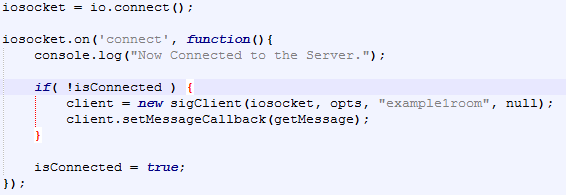
\includegraphics[width=0.9\textwidth]{backend/Modul_UserClientHowTo.PNG}
\caption{Verwendung Client}
\label{backfig11}
\end{figure}
In Abbildung \ref{backfig11} ist zu sehen, wie das Modul auf Clientseite genutzt werden kann.
Vorbedingung ist, dass wie zu sehen, eine Verbindung des socket.io WebSocket besteht.
Sobald diese besteht kann ein neues "sigClient" Objekt erstellt werden.
Diesem müssen vier Parameter übergeben werden:

\begin{description}
\item[Socket]
Der verbundene "socket.io"-Socket.

\item[Opts]
Etwaiige Optionen, alle optional. Mehr dazu unter \ref{moduleoptions}.

\item[Roomname]
Der Name des Raums, dem der Client beitreten will.

\item[Placeholder]
Ein Platzhalter für mögliche Zweitmodi.
\end{description}



\subsubsection{Nachricht Empfangen}
\begin{figure}[htH]
\centering
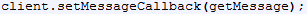
\includegraphics[width=0.9\textwidth]{backend/Modul_UserClientHowToMessageCallback.PNG}
\caption{Client Nachricht empfangen}
\label{backfig12}
\end{figure}
In Abbildung \ref{backfig12} ist zu sehen, wie eine Callback Funktion für neue Nachrichten gesetzt wird. 
Diese Funktion wird immer dann aufgerufen, wenn eine neue Nachricht empfangen wurde. Näheres zu der Struktur von Nachrichten unter \ref{messagestructure}.



\subsubsection{Nachricht Senden}
\begin{figure}[htH]
\centering
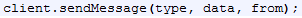
\includegraphics[width=0.9\textwidth]{backend/Modul_UserClientHowToSendMessage.PNG}
\caption{Client Nachricht senden}
\label{backfig13}
\end{figure}
In Abbildung \ref{backfig13} ist zu sehen, wie eine Nachricht versendet werden kann.
Beim Versenden einer Nachricht sind zwei Parameter von relevanz:

\begin{description}
\item[Type]
Der Typ der Nachricht. Vom Nutzer frei wählbar. Dient der schnellen Zuordnung.

\item[Data]
Die Nutzlast der Nachricht. Hierbei ist hervorzuheben, dass dies Nutzlast im Format eines JavaScript Objektes sein sollte. Sollte eine Verbindung mit WebRTC nicht hergestellt werden und der Backup-Modus ist aktiviert und unterstützt, kann dem Data-Objekt ein "to" Attribut hinzugefügt werden, welches die ID des Empfängers enthält um dem Server mitzuteilen, für wen diese Nachricht gedacht war.
\end{description}



\subsection{Verwendung des Server}
\subsubsection{Abhängigkeiten}
\begin{figure}[htH]
\centering
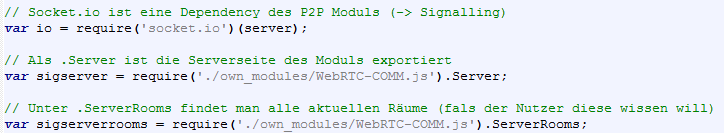
\includegraphics[width=0.9\textwidth]{backend/Modul_UserServerDependencies.PNG}
\caption{Dependencies Verwendung Server}
\label{backfig6}
\end{figure}
In Abbildung \ref{backfig6} ist zu sehen, welche Abhängigkeiten auf Serverseite bestehen.
Für das Signalling nutzt das Modul die Serverseitige Implementation von "socket.io". 
Zur Nutzung des Moduls muss dieses außerdem "required" werden. Hierzu wird der Pfad zu dem Modul als Parameter an das require übergeben und der Server Export genutzt.
Die Verwendung der ServerRooms ist optional und gibt dem Nutzer die Möglichkeit auf dem Server eine Einsicht in die derzeitigen Räume zu erlangen und über WebSockets die in diesen hinterlegt sind mit den Clients zu Kommunizieren.



\subsubsection{Konstruktor}
\begin{figure}[htH]
\centering
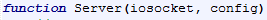
\includegraphics[width=0.9\textwidth]{backend/Modul_ServerContructor.PNG}
\caption{Server Konstruktor}
\label{backfig7}
\end{figure}
In Abbildung \ref{backfig7} ist der allgemeine Konstruktor des Moduls für Server zu sehen.



\subsubsection{Allgemeine Verwendung} \label{serveruse}
\begin{figure}[htH]
\centering
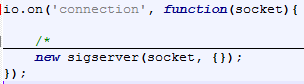
\includegraphics[width=0.9\textwidth]{backend/Modul_UserServerHowTo.PNG}
\caption{Nutzung Server}
\label{backfig8}
\end{figure}
In Abbildung \ref{backfig8} ist zu sehen, wie das Modul für Server genutzt wird. Für jeden neuen Client der sich erfolgreich mit dem Server verbunden hat muss ein neues Modul.Server Objekt erstellt werden. An dieses Modul muss der Socket (socket.io) und etwaige optionale Parameter/Optionen übergeben werden. Die Erstellung dieses Objektes führt dazu, dass Eventhandler des WebSocket für das Handling des Signalling erstellt werden und der Nutzer einem Raum zugewisen werden kann. Dies geschieht alles automatisch und intern im Modul. Der in Abbildung \ref{backfig8} zu sehende Code stellt die Minimalimplementation dar, wie sie auch im Projekt "Ping-Pong" verwendet wird. In den meisten Fällen reicht diese aus.



\subsection{Verwendung der Callbacks} \label{callbacks}
Alle wichtigen Ereignisse, welche den reibungslosen Aufbau und Betrieb der Verbindung betrifft, wird intern geregelt. Dem Nutzer des Moduls ist es jedoch möglich, eigene Callbacks zu definieren, die bei gewissen Ereignissen aufgerufen werden.
\begin{figure}[htH]
\centering
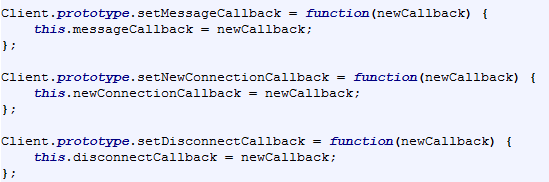
\includegraphics[width=0.9\textwidth]{backend/Modul_Callbacks.PNG}
\caption{Callbacks}
\label{backfig9}
\end{figure}
In Abbildung \ref{backfig9} sind die drei für den Nutzer wichtigsten Funktionen zum Eintragen von Callbacks zu erkennen.

\begin{description} \label{messagestructure}
\item[setMessageCallback]
Mit dieser Funktion trägt man eine Callback Funktion ein, die Falle einer neuen Nachricht aufgerufen wird. 
Die Callback Funktion wird hierbei mit drei Parametern aufgerufen:

  \begin{description}
  \item[Type]
  Dem Typen den die Nachricht hat, vergeben von dem Sender.
  
  \item[From]
  Der ID des Absenders der Nachricht.
  
  \item[Data]
  Die eigentliche Nutzlast der Nachricht. Format vom Sender bestimmt.
  \end{description}

\item[setNewConnectionCallback]
Mit dieser Funktion trägt man eine CallbackFunktion  ein, die im Falle einer neuen erfolgreichen Verbindung zu einem anderen Peer aufgerufen wird.
Die Callback Funktion wird hierbei mit einem Parameter aufgerufen:

  \begin{description}
  \item[PeerID]
  Die ID des neuen Peers.
  \end{description}
  
\item[setDisconnectCallback]
Mit dieser Funktion trägt man eine Callback Funktion ein, die im Falle des Verbindungsverlusts eines Peers aufgerufen wird.
Die Callback Funktion wird hierbei mit einem Parameter aufgerufen.

  \begin{description}
  \item[PeerID]
  Die ID des Peers, welcher die Verbindung verloren hat.
  \end{description}
\end{description}



\subsection{Verwendung der Optionen} \label{moduleoptions}
\begin{description}
\item[Client]
Beim Erstellen eines Client-Objektes können gewisse Optionen mit übergeben werden. Hierbei kann eine beliebige Anzahl dieser genutzt werden. Wird eine Option nicht genutzt, tritt ein default in Kraft (default mit = markiert):
\begin{quote}
  \begin{description}
  \item[mode (=single|multi)]
  Der Modus, den der Peer nutzen soll.
  
  \item[maxpeers (=1|1..2^3^2-1]
  Die Anzahl der maximal möglichen gleichzeitigen Verbindungen. (Relevant für "Multi-Peer")

  \item[usebackup (=false|true)]
  Die Möglichkeit der Verwendung von WebSockets als Backup. Diese option muss der Server auch Unterstzützen.
  \end{description}
\end{quote}

\item[Server]
Beim Erstellen eines Server-Objektes können gewisse Optionen mit übergeben werden.
Hierbei kann eine beliebige Anzahl dieser genutzt werden.
Wird eine Option nicht genutzt, tritt ein default in Kraft (default mit = markiert):
\begin{quote}
  \begin{description}
  \item[allowtopology_star (=true|false)]
  Sterntopologie erlauben.
  
  \item[allowtopology_1v1 (=true|false)]
  Eins zu eins "Topologie" erlauben.
  
  \item[allowtopology_ava (=false|true)]
  Vollvermaschung erlauben. Default ist false, da hierdurch auch für den Server eine große Last durch die vielen Signale entstehen kann.  
  
  \item[usebackup (=false|true)]
  Die Möglichkeit der Verwendung von WebSockets als Backup. Kann sehr Performaceintensiv werden.
  \end{description}
\end{quote}
\end{description}



\section{Eigenes Modul: Performance}
\subsection{Testbedingungen}
Diese Tests dienen ausschließlich der bewertung und Bildung eines Leistungsschemas für das Modul. Aus diesem Grund wurde der Faktor Netzwerk auf ein minimum begrenzt und nur Computer in einem LAN verwendet. Folge daraus ist, dass die Adressen dem LAN zugeordnet werden konnten und ein Routing außerhalb des LAN nicht nötig war. Eine durchschnittliche Latenz von ~1ms war gegeben (laut Anzeige, Messung erfolgte im ms Bereich). 
Ablauf eines jeden Tests:

\begin{enumerate}
\item
Es wurde ein Node.JS Server mit Minimalimplementation des Moduls gestartet. (Für Minimalimplementation siehe \ref{serveruse})

\item
Ein einzelner ''Multi-Peer'' wurde gestartet. Dieser tritt einem Testraum bei.

\item
Mit Hilfe eines kleinen Test-Programms wurde eine gewisse Anzahl an ''Single-Peer'' Sendern gestartet und via WebRTC mit dem "Multi-Peer" Host im gleichen Raum verbunden.

\item
Nachdem alle Peers erfolgreich verbunden sind wird eine Startzeit des Tests gespeichert.

\item
Die Sender fangen nun an in einer gewissen Frequenz bestimmt oft eine Nachricht an den ''Multi-Peer'' zu senden.
Die Payload dieser Nachricht besteht aus:
  \begin{description}
  \item[ID]
  Die eigene ID. Nötig da mehrere Sender auf einem System befindlich sind und nur so die zuordnung der Ergebnisse möglich ist.
  
  \item[Time]
  Ein Zeitstempel der direkt zum Sendezeitpunkt generiert wurde.
  
  \item[Index]
  Ein Index der für ID der versendeten Nachricht steht.
  \end{description}

Aus ID und Index lässt sich eine Nachricht exakt zuweisen.

\item
Empfängt der ''Multi-Peer'' eine Nachricht schickt er diese einfach direkt zum Absender zurück.

\item
Empfangt einer der ''Single-Peer'' eine Nachricht, tragen sie in ein Ergebnisobjekt den Sende- und Empfangszeitpunkt ein.

\item
Sind alle Sender mit ihren Sende-Iterationen durch und es wurde die gleiche Anzahl an Nachrichten wieder empfangen (Anzahl der Ergebnisobjekte), wird wieder ein Zeitstempel generiert.

\item
Nachdem Sende- und Empfangszyklen durch sind werden die Ergebnisobjekte ausgewertet. Dabei wird ermittelt:

  \begin{description}
  \item[Gesamtlaufzeit]
  Ermittelt aus Start- und Endzeitpunkt.
  
  \item[Gesamtzahl der Nachrichten]
  Anzahl aller empfangenen Nachrichten.
  
  \item[Minimale Delay]
  Kleinste bei einer Nachricht ermittelte Verzögerung.
  
  \item[Maximale Delay]
  Größte bei einer Nachricht ermittelte Verzögerung.
  
  \item[Durchschnittliche Delay]
  Mittelwert aller ermittelten Verzögerung.
  
  \item[Zeit pro Nachricht]
  Zeitabstand zwischen Nachrichten.
  \end{description}

\item
Wiederhole Test noch 9 mal und mittle Ergebnisse.
\end{enumerate}



\subsubsection{Erfolgskriterien}
\begin{description}
\item[Hard]
Das Harte Kriterium ist, dass das Maximale Delay nicht über der Zeit pro Nachricht liegen darf. Die Nachricht eines jeden Senders wurde also verarbeitet und beantwortet, bevor er eine neue sendet.

\item[Soft]
Das Weiche Kriterium ist, dass das durchschnittliche Delay nicht über der Zeit pro Nachricht liegen darf. Die Nachricht eines jeden Sendern wurde also in der Regel verarbeitet und beantwortet, bevor er eine neue sendet.

\item[Failed]
Sobal das weiche Kriterium nicht mehr erfüllt ist, ist ein Erfolg im allgemeinen nicht mehr gegeben. Je nach Anwendungsfall kann auch ein Failed noch ausreichend sein und es müssten speziellere Kriterien herangezogen werden.
\end{description}



\subsection{Allgemeiner Performanceaspekt} \label{associativearray}
Bei diesen Tests sollte berücksichtigt werden, dass der Verarbeitungsaufwand nach erhalt der Nachrichten sich lediglich auf das richtige weiterleiten der Nachricht beschränkt. 
Dabei wird die Nachricht an eine Callback Funktion weitergereicht und dann eine neue Nachricht an einen Peer versendet. 
Tragend für die Performance ist hier die Verwaltung der Verbindungen.
Alle Verbindungen werden in ''assoziativen'' Arrays verwaltet. Da ein ''assoziatives'' Array in JavaScript eigentlich nicht existiert, sind dies Objekte mit Attributen. 



\subsubsection{Lookup}
Je nach Browser kann das ''lookup'' verschiedene Aufwände annehmen.
Bei modernen Browsern kann von einem Worst-Case von \mathcal O\left( log_{ 2 }\left( N \right) \right) ausgegangen werden.
Bei modernen Browsern kann von einem Best-Case von \mathcal O\left( 1 \right) ausgegangen werden.
Bei älteren Browsern kann von einem Worst-Case von \mathcal O\left( N \right) ausgegangen werden.



\subsubsection{Zuweisung}
Zuweisung von Werten auf bereits bestehende Attribute von Objekten fällt unter gleichen Aufwand wie ''lookup''.
Zuweisung von Werten auf neue Attribute hat einen Aufwand von \mathcal O\left( 1 \right) im Best-Case bis \mathcal O\left( N \right) im Worst-Case je Browserimplementation. In modernen Browsern ist von \mathcal O\left( 1 \right) auszugehen.



\subsubsection{Concurrency}
Concurrency ist mit JavaScript unter den hier genutzten Techniken nicht möglich, somit müssen keine Synchronisationsmechanismen untersucht werden.




\subsection{Performance: Beispiel am Projekt}

\subsubsection{Beschreibung}
Dieser Test soll die Bedingungen des Projektes wiederspiegeln.



\subsubsection{Durchführung}
\begin{quote}
  \begin{description}
  \item[Anzahl Sender]
  Als Anzahl der Sender für die Versuche wurde festgelegt: 2, 3, 4, 6, 10, 15, 25, 50, 75, 100, 125, 150.
  
  \item[Frequenz der Nachrichten]
  Jeder Sender sendete 20 Nachrichten pro Sekunde, also alle 50ms eine Nachricht.
  
  \item[Iterationsgröße]
  Jeder Sender sendete 600 Nachrichten.
  
  \item[Folge: Nachrichtendurchsatz]
  Aus Anzahl der Sender und Frequenz entstand folgender Durchsatz(in Nachrichten/s): 40, 60, 80, 120, 200, 300, 500, 1000,     1500, 2000, 2500, 3000.
  \end{description}
\end{quote}



\subsubsection{Ergebnis}
\begin{figure}[htH]
\centering
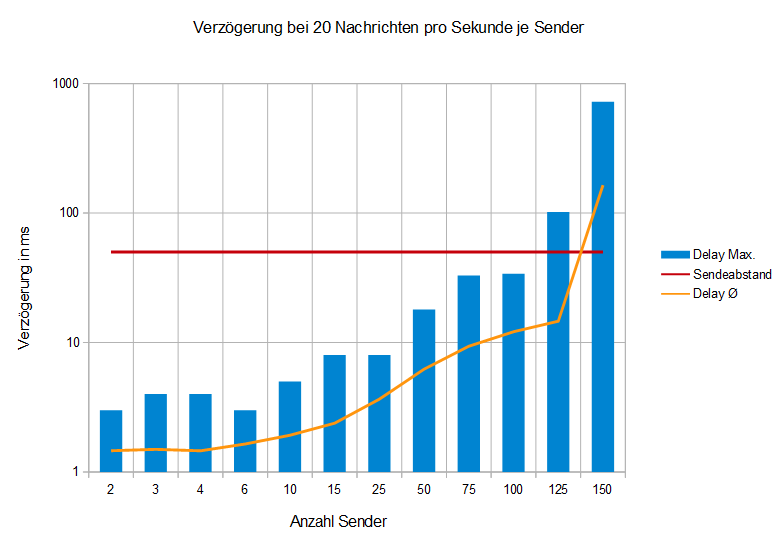
\includegraphics[width=0.9\textwidth]{backend/Diagramm_Performance_Normal.PNG}
\caption{Diagramm Performancetest Normal}
\label{backfig14}
\end{figure}
In Abbildung \ref{backfig14} ist das Ergebnis der Tests zu erkennen. 
Auf der Y-Achse ist die Verzögerung logarithmisch skaliert in ms dargestellt.
Auf der X-Achse ist die Anzahl der Sender dargestellt.
Die Balken stellen die maximale Verzögerung dar. 
Die gelbe Linie stellt die durchschnittliche Verzögerung dar.
Die rote Linie stellt die Sende-Verzögerung pro Nachricht dar.
Befindet sich ein Balken über der roten Linie ist das ''Hard''-Kriterium nicht mehr erfüllt.
Befindet sich die gelbe Linie über der roten Linie ist das ''Soft''-Kriterium nicht mehr erfüllt.



\subsubsection{Fazit}
\begin{figure}[htH]
\centering
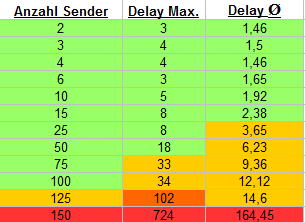
\includegraphics[width=0.9\textwidth]{backend/Tabelle_Performance_Normal.PNG}
\caption{Tabelle Performancetest Normal}
\label{backfig15}
\end{figure}
In Abbilding \ref{backfig15} ist das Ergebnis noch einmal Tabellarisch dargestellt.
Zu erkennen ist, dass das ''Hard''-Kriterium noch bis 100 Peers erfüllt ist. Dies entsrpicht einem Nachrichtendurchsatz von 2000 Nachrichten pro Sekunde. Das ''Soft''-Kriterium ist noch bis 125 Peers erfüllt. Dies entspricht einem Nachrichtendurchsatz von 2500 Nachrichten pro Sekunde. Markante Punkte:
\begin{quote}
  \begin{description}
  \item[25 Sender]
  Bei der Steigerung von 15 auf 25 Sender steigt die maximale Verzögerung nicht, jedoch die durchschnittliche Verzögerung um 53%.

  \item[75 Sender]
  Bei 75 Sendern erreicht die maximale Verzögerung zum ersten mal mehr als 50\% des ''Soft''-Kriterium.

  \item[125 Sender]
  Bei 125 Sendern ist das ''Hard''-Kriterium nicht mehr erfüllt.

  \item[150 Sender]
  Bei 150 Sendern ist das ''Soft''-Kriterium nicht mehr erfüllt.
  \end{description}
\end{quote}

Bezogen auf das Ping-Pong Projekt, welches Spieler-/Peerzahlen unter 10 nutzt, sind keine Auffälligkeiten zu erkennen und sowohl ''Soft''- als auch ''Hard''-Kriterium sind erfüllt.




\subsection{Performance: Beispiel für Chat}

\subsubsection{Beschreibung}
Folgender Test nimmt sich eine Chat-Anwendung als Beispiel.



\subsubsection{Durchführung}
\begin{quote}
  \begin{description}
  \item[Anzahl Sender]
  Als Anzahl der Sender für die Versuche wurde festgelegt: 50, 100, 150, 200, 250.

  \item[Frequenz der Nachrichten]
  Jeder Sender sendete 1 Nachricht pro Sekunde, also alle 1000ms eine Nachricht.

  \item[Iterationsgröße]
  Jeder Sender sendete 30 Nachrichten.

  \item[Folge: Nachrichtendurchsatz]
  Aus Anzahl der Sender und Frequenz entstand folgender Durchsatz(in Nachrichten/s): 50, 100, 150, 200, 250.
  \end{description}
\end{quote}



\subsubsection{Ergebnis}
\begin{figure}[htH]
\centering
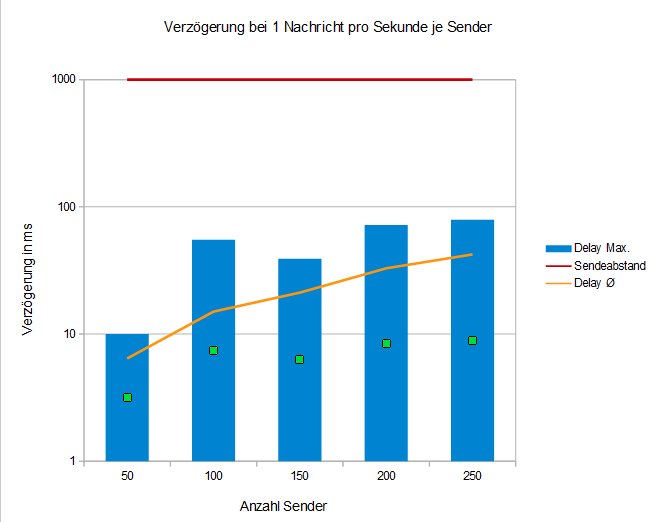
\includegraphics[width=0.9\textwidth]{backend/Diagramm_Performance_Chat.PNG}
\caption{Diagramm Performancetest Chat}
\label{backfig16}
\end{figure}
In Abbildung \ref{backfig16} ist das Ergebnis der Tests zu erkennen. 
Auf der Y-Achse ist die Verzögerung logarithmisch skaliert in ms dargestellt.
Auf der X-Achse ist die Anzahl der Sender dargestellt.
Die Balken stellen die maximale Verzögerung dar. 
Die gelbe Linie stellt die durchschnittliche Verzögerung dar.
Die rote Linie stellt die Sende-Verzögerung pro Nachricht dar.
Befindet sich ein Balken über der roten Linie ist das ''Hard''-Kriterium nicht mehr erfüllt.
Befindet sich die gelbe Linie über der roten Linie ist das ''Soft''-Kriterium nicht mehr erfüllt.



\subsubsection{Fazit}
\begin{figure}[htH]
\centering
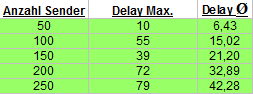
\includegraphics[width=0.9\textwidth]{backend/Tabelle_Performance_Chat.PNG}
\caption{Tabelle Performancetest Chat}
\label{backfig17}
\end{figure}
In Abbildung \ref{backfig17} ist das Ergebnis noch einmal Tabellarisch dargestellt.
Zu erkennen ist, dass auch bei 250 Sendern noch die ''Soft''- und ''Hard''-Kriterien erfüllt sind.
Ein Test mit mehr Peers stellte sich als problematisch da, da der Browser je nach Implementation bei einer großen Anzahl gleichzeitiger Verbindungen anfängt einzelne Verbindungen, die eine Weile nicht genutzt wurden, zu schließen. Dies trat auch auf, da die Initialisierungsphase des Tests diese Inaktivitätsschwälle überschritt. 
Gleichmäßige Testdurchläufe waren nicht mehr möglich.
Bester Einzeldurchlauf: 950 Peers. Inkonsistent.

Chatanwendungen auf dieser Basis stellen theoretisch keine Probleme dar.



\subsection{Performance: Beispiel extreme}
\subsubsection{Beschreibung}
Das extreme Beispiel soll zeigen, wie sich eine hohe Sendefrequenz auswirkt. Beispiel hierfür soll sein, dass Steuerdaten zu jedem Bild verarbeitet werden sollen. Hierbei markant, es soll sich um einen 144Hz Monitor handeln. (Aufgrund Rundung: 142.85Hz)



\subsubsection{Durchführung}
\begin{quote}
  \begin{description}
  \item[Anzahl Sender]
  Als Anzahl der Sender für die Versuche wurde festgelegt: 20, 25, 30, 35, 40.

  \item[Frequenz der Nachrichten]
  Jeder Sender sendete 142.85 Nachricht pro Sekunde, also alle 7ms eine Nachricht.

  \item[Iterationsgröße]
  Jeder Sender sendete 4320 Nachrichten.

  \item[Folge: Nachrichtendurchsatz]
  Aus Anzahl der Sender und Frequenz entstand folgender Durchsatz(in Nachrichten/s): 2857, 3571.25, 4285.5, 4999.75, 5714.
  \end{description}
\end{quote}



\subsubsection{Ergebnis}
\begin{figure}[htH]
\centering
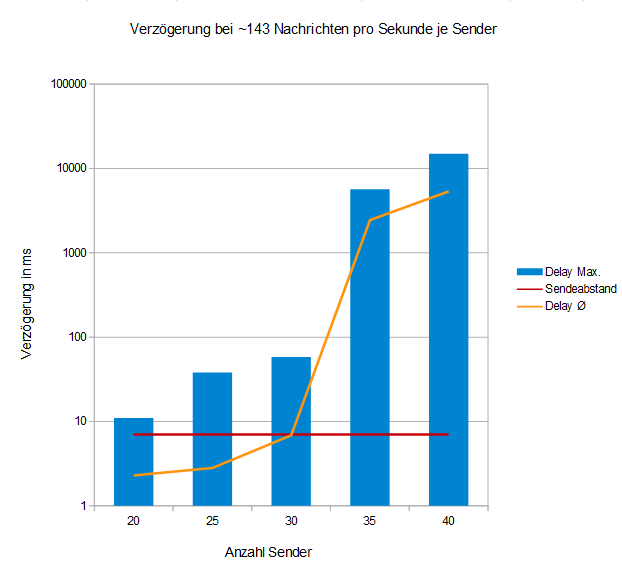
\includegraphics[width=0.9\textwidth]{backend/Diagramm_Performance_144hz.PNG}
\caption{Diagramm Performancetest 144Hz}
\label{backfig18}
\end{figure}
In Abbildung \ref{backfig16} ist das Ergebnis der Tests zu erkennen. 
Auf der Y-Achse ist die Verzögerung logarithmisch skaliert in ms dargestellt.
Auf der X-Achse ist die Anzahl der Sender dargestellt.
Die Balken stellen die maximale Verzögerung dar. 
Die gelbe Linie stellt die durchschnittliche Verzögerung dar.
Die rote Linie stellt die Sende-Verzögerung pro Nachricht dar.
Befindet sich ein Balken über der roten Linie ist das ''Hard''-Kriterium nicht mehr erfüllt.
Befindet sich die gelbe Linie über der roten Linie ist das ''Soft''-Kriterium nicht mehr erfüllt.



\subsubsection{Fazit}
\begin{figure}[htH]
\centering
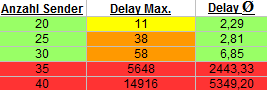
\includegraphics[width=0.9\textwidth]{backend/Tabelle_Performance_144hz.PNG}
\caption{Tabelle Performancetest 144Hz}
\label{backfig19}
\end{figure}
In Abbildung \ref{backfig19} sind die Ergebnisse noch einmal Tabellarisch dargestellt.
Zu erkennen ist, dass das ''Hard''-Kriterium schon bei 20 Sendern nicht mehr erfüllt ist.
Außerdem zu erkennen ist, dass ab 35 Sendern auch das ''Soft''-Kriterium nicht mehr erfüllt ist.

Markante Punkte:

\begin{quote}
  \begin{description}
  \item[20 Sender]
  Bei 20 Sendern ist das ''Hard''-Kriterium nicht mehr erfüllt, die durchschnittliche Verögerung aber noch sehr gut.

  \item[25 Sender]
  Im Gegensatz zu 20 Sendern, hat sich bei 25 Sendern die Maximale Verzögerung um 245\% auf 38ms erhöht. Anzeichen für einen zeitweisen Nachrichtenstau.

  \item[30 Sender]
  Im Gegensatz zu 25 Sendern, hat sich bei 30 Sendern die durchschnittliche Verzögerung um 143\% auf 6.85ms erhöht. Ein Zeichen dafür, dass immer öfter Nachrichtenstaus auftreten.

  \item[35 Sender]
  Im Gegensatz zu 30 Sendern, hat sich bei 35 Sendern die maximale Verzögerung um 9637\% auf 5648ms und die durchschnittliche Verzögrung um 35569\% auf 2443.33ms erhöht. Hierbei ist von einem Durchgängig anwachsendem Nachrichtenstau auszugehen.

  \item[40 Sender]
  Noch einmal hat sich im Gegensatz zu 35 Sendern bei 40 Sendern die Verzögerung noch einmal vervielfacht.
  \end{description}
\end{quote}

Sofern das ''Hard''-Kriterium kein muss ist, können solche Mengen an Nachrichten noch bis 30 Sender verarbeitet werden.



\section{Eigenes Modul: Möglichkeiten}

\subsection{Verwendbarkeit}
Das Modul ist wie im Projekt genutzt getestet und verwendbar. 
Es ist generisch nutzbar.
Einige zusätzliche Features, welche auch für das Projekt nicht von Relevanz waren, sind nur teilweise implementiert oder nicht getestet. 
Dies ist auf den großen Umfang eines solchen Modules zurückzuführen. \\ \\
Bei diesen teilweise implementierten Features handelt es sich um:
\begin{enumerate}
\item
Interaktiven Raumwechsel.

\item
Benutzerspezifische Sendekanäle.

\item
Echtzeit Verbindungsanalysen.
\end{enumerate}
\\ \\
Bei den nicht ausführlich getesteten Features handelt es sich um:
\begin{itemize}
\item
Topologie Eins-zu-Eins und Vollvermascht. Grund ist, dass hierfür weitere Testanwendungen nötig wären.

\item
Backup funktionalität über WebSocket. Grund ist, dass ein Test in verschiedenen Netzen noch erfolgen muss.
\end{itemize}


\subsection{Erweiterbarkeit}
\begin{itemize}
\item
Angesichts der verschiedenen möglichen Topologien gibt es für die Peers nur zwei verschiedene Verhalten. 
Entweder sie pflegen nur eine Verbindung, oder mehrere.
Da dieses Verhalten bereits modelliert ist, ist die implementation neuer Topologien auf Serverseite zu geschehen, welche die Räume verwaltet.

\item
Als Verbindungsobjekte werden unveränderte RTCPeerConnections verwendet, wodurch das hinzufügen neuer Datenkanäle ein neues Verwalungsobjekt auf Clientseite benötigen würde.
Außerdem müssten die verschiedenen Datenkanäle entweder auf mehrere Callback Funktionen gemapped werden, oder ein Parameter für die eine Callback Funktion definiert werden, welche die Datenkanäle logisch trennt.

\item
Für die Implementation von Speziellen Datenkanälen, wie z.B. Medienkanälen, muss ähnlich wie bei den normalen Datenkanälen, ein Verwaltungsobjekt geschaffen werden, und etwaiige Callback Funktionen bestimmt.

\item
Die Implementation eines Senderelays (A, B, C und D sind Peers. A sendet an D über B und C: A->B->C->D) liegt in Nutzerhand. Es müsste eine Implementation stattfinden bei dem ein Client (B und C) zwei Verbindungen herstellt. 
Dabei pflegt B jeweils eine zu A und C, C jeweils zu B und D.
Ankommende Nachrichten müssten dann an die andere Verbindung weitergereicht werden.
Diese Nutzer-Implementation könnte dann auch die Teilvermaschung ermöglichen.
\end{itemize}



\section{Fazit der Arbeit am Modul}
Die große Fehlermenge anderer Module zeigt, wie komplex ein genau definiertes Thema sein kann.
Etliche verschiedene kleine Abweichungen der Browserspezifischen WebRTC-Implementationen führen dazu, dass auf viele ''Marotten'' eingegangen werden muss.
Auch wenn dieses Modul einen bis dato guten Ansatz liefert, fehlen noch viele bereits beschriebene Features, um dieses Modul ein vollständiges nennen zu können.
Die Erstellung eines solchen Moduls ist vom Umfang her größer einzuordnen, als anfänglich erwegt. 
Viele Refactoringschritte wurden nicht durchgeführt, dar der Zeitliche Aspekt dieses Projektes dies nicht mehr zu ließ.

\chapter{Frontend}
\section{Ideensammlung}
In diesem Teil finden alle Ideen und Gedanken zu dem Projekt Platz welche ich vor Projektbeginn hatte.
\subsection{Allgemeine Ideen}
\paragraph{Partikeleffekte}
\mbox{}\\
Bei Kollision des Balles mit den Wänden, den Schlägern oder gar anderen Bällen wäre ein Partikeleffekt sehr schön.
\newline
Ebenfalls könnte man mit Partikeleffekten den Ballverlust (Zerstörung des Balles in den "Toren") sehr schön grafisch unterstreichen.
\newline
Möglicherweise dafür geeignete Engine:
\href{http://soulwire.github.io/sketch.js/}{Sketch.js}
\paragraph{Multiplayer}
\mbox{}\\
Ideen zu Spielen mit mehr als 2 Spielern.
\begin{itemize}
	\item Punkt bei Ballverlust erhält der letzte Spieler. Spiel merkt sich letzte 2 Ballkontakte sodass der Abschläger erkannt werden kann.
	\item Spieler \& Ball färben. Man könnte die Schläger Färben und die Bälle bei Ballkontakt der eigenen Farbe zuweisen. So erhalten die Spieler einen Visuellen Indikator wer Punkte bekommen kann.
\end{itemize}
\newpage
\paragraph{Schläger}
\begin{itemize}
\item
\textbf{Bewegung des Schlägers} Bewegung kann Relativ oder Absolut erfolgen. Bei absoluter Bewegung wird der Schläger sehr stark springen und möglicherweise das Spiel zu einfach werden.
\item
\textbf{Geschwindigkeit} Man sollte die Geschwindigkeit des Schläger begrenzen sodass das Spiel  schwieriger wird.
\item
\textbf{Begrenzung} Der Schläger braucht 2 Begrenzungen damit er das Spielfeld nicht verlässt.
\item
\textbf{Input der Controller} Der Input sollte so einfach wie möglich gestaltet werden. Am besten nur die Richtung und die Positionsänderung übertragen.
\end{itemize}
\subsection{Spielfelder}
\paragraph{Original Pong}
\mbox{}\\
Im Orinalen Pong betrugen die Abmaße der Komponenten folgende werte:
\begin{itemize}
	\item
	      Spielfeld Größe: 512*256px
	\item
	      Ball 6*5px
	\item
	      Schläger 2*28px
	\item
	      Schläger Geschwindigkeit 4px pro Intervall
\end{itemize}
\newpage
\paragraph{2 Spieler Normal}
\mbox{}\\
\begin{figure}[ht]
	\begin{center}
		\makebox[\textwidth]{
\includegraphics[width=300pt]{frontend/Ping-Pong-2p.png}}
	\end{center}
	\caption{Mockup eines 2-Spieler Feldes}
	\label{figx}
\end{figure}
\newline
\paragraph{2 Spieler Breakout}
\mbox{}\\
Die Idee für dieses Feld war es 2 Klassiker miteinander zu verbinden. Die Spieler zerstören mit einem eigenen Ball die Felder. Das Spiel endet wenn alle Felder zerstört sind. Gewinner ist der Spieler welcher mehr Felder zerstört hat.
\newline
Die Spieler sollten nur den eigenen Ball beeinflussen können. Also muss für den jeweils anderen Spieler eine Barriere errichtet werden.
\newline
\begin{figure}[ht]
	\begin{center}
		\makebox[\textwidth]{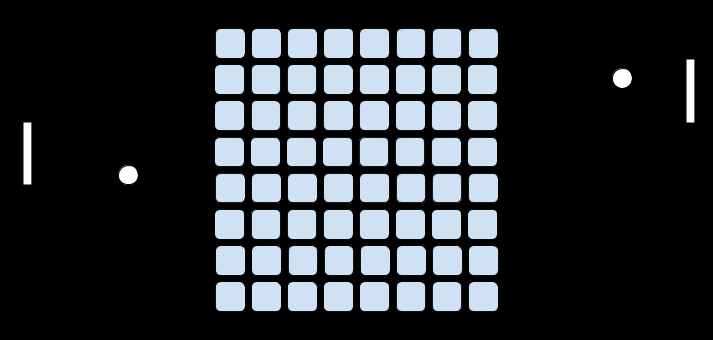
\includegraphics[width=300pt]{frontend/Ping-Pong-Breakout.png}}
	\end{center}
	\caption{Mockup eines 2-Spieler Feldes im Spielmodus Breakout}
	\label{figx}
\end{figure}
\newpage
\paragraph{3 Spieler}
\mbox{}\\
Als ich die Präsentation des Projektes sah war ich nicht mit den Ideen für einen Multispielermodus zufrieden. Sofort kam mir folgende Idee:
\newline
3 Spieler spielen in einem abgeschnittenem Dreieck, bzw eines gleichseitigen Sechseckes. Jeder kontrolliert eine Seite.
\newline
\begin{figure}[ht]
	\begin{center}
		\makebox[\textwidth]{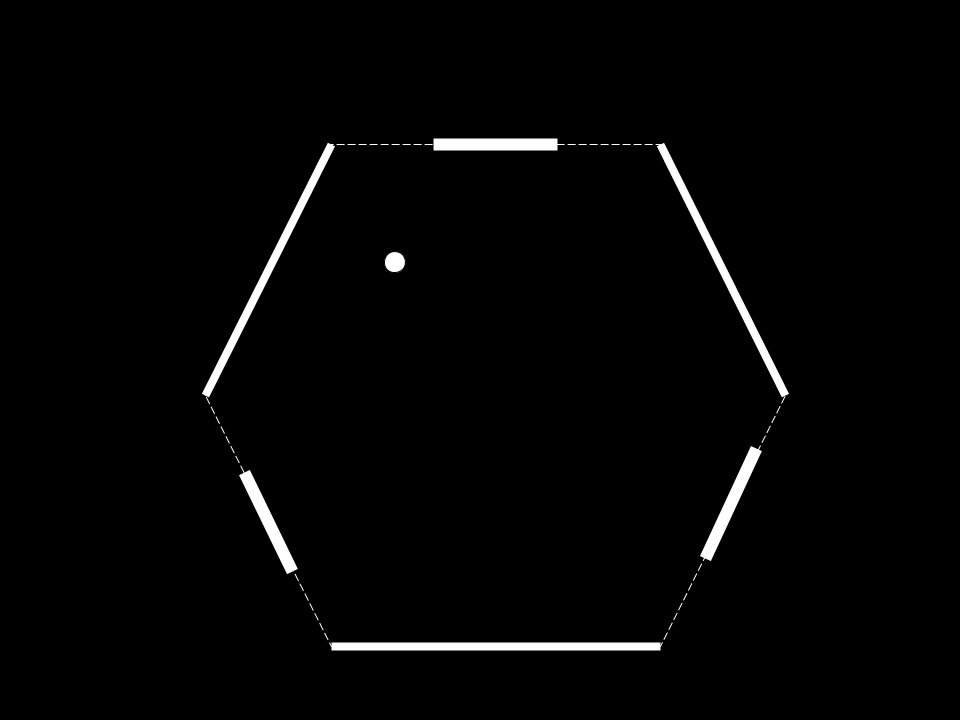
\includegraphics[width=300pt]{frontend/Ping-Pong-3p.png}}
	\end{center}
	\caption{Mockup eines 3-Spieler Feldes}
	\label{figx}
\end{figure}
\newline
\paragraph{4 Spieler}
\mbox{}\\
Als weitere Idee kam mir ein Vier-Spieler Feld bei dem sich in einem Quadrat je 2 Spieler gegenüberstehen.
\newline
Mehr als 4 Spieler sind meiner Meinung nach nicht notwendig. Wenn man bedenkt das sich die Spieler vor einem Bildschirm im Flur sammeln.
\newline
Denkbar ist allerdings das man das Konzept für 3 und 4 Spieler für weitere Spieler weiterführt.
\newpage
\subsection{Power-Ups}
Kurze Ideensammlung zu möglichen Verstärkungen.
\begin{itemize}
	\item
	      \textbf{Magnet:} Ball wird vom Schläger angezogen. Der Spieler erhält dann die Möglichkeit den Ball zu führen und gezielt abzustoßen.
	\item
	      \textbf{Größerer / Kleinerer Ball:} Ball-Modifikator, denkbar auch eine pulsierende Variante wobei sich der Ball durchgehend in der Größe verändert.
	\item
	      \textbf{Multi-Ball:} Ball wir mehrfach dupliziert. Die verschiedenen Bälle fliegen vom Startpunkt aus in alle Richtungen und zählen alle als normaler Ball. Bei Ballverlust tauchen diese nicht erneut auf.
	\item
	      \textbf{Steuerung Invertieren:} Steuerung des Gegners wird invertiert.
	\item
	      \textbf{Geschwindigkeitsmodifikation des Schlägers:} Eigener Schläger wird schneller oder gegnerischer wird langsamer.
\end{itemize}
\subsection{Statistiken}
Auflistung an Daten welche für eine Statistik relevant wären.
\begin{itemize}
	\item
	      Spieldauer
	\item
	      Ballkontakte je Spieler
	\item
	      Zurückgelegte Distanz des Balles
	\item
	      Zurückgelegte Distanz je Spieler
	\item
	      Genauigkeit der Schläger
	      \newline
	      (Ballkontakte / Durchgelassene Bälle)
\end{itemize}
\newpage
\section{Auswahl einer Physics-Engine}

\begin{quote}
	\href{https://github.com/Transport-Protocol/MBC-Ping-Pong/issues/3}{Auswahl einer geeigneten 2D-/Physiksengine \#3}
	\newline
	Die Darstellung auf dem Anzeigegerät ist über den DOM nicht möglich, da die Bewegung des Balls und der Schläger zu schnell werden. Zudem wird auch die Physik auf dem Anzeigegeräts berechnet. Hierfür ist eine Kollisionserkennung erforderlich.
\end{quote}
Für die physikalisch korrekte Kollision des Balles mit der Spielwelt und den Schlägern haben wir uns entschieden eine Physics-Engine zu verwenden.

\subsection{Matter.JS}
Matter js ist eine sehr mächtige Engine. Sie unterstützt viele Formen und Physikalische Eigenschaften wie zum Beispiel Masse und wirkende Kräfte auf die jeweiligen Objekte. 
Es besteht die Möglichkeit physikalische Objekte zusammen zusetzen und sogar diese Elastisch erscheinen zu lassen, so ist es beispielsweise möglich Stoff oder schwingende Seile zu erstellen.
Nach mehrstündiger Einarbeitung kam ich zu dem Schluss das diese Engine für unser Projekt nicht geeignet ist.
Gründe hierfür sind:
\begin{itemize}
	\item
	      Zu Komplex:
	      Die Einrichtung des Spielfeldes erwies sich als überaus schwierig. Gute Anleitungen für einfache Szenarien fehlten, die verfügbaren Anleitungen sind zu grundlegend beschrieben.
	      Ebenfalls half die Anleitung der Engine nicht bei der Verwendung der einzelnen Komponenten.
	\item
	      Die Positionierung der Objekte bezog sich immer auf den Mittelpunkt des Objektes, man kann beispielsweise kein Rechteck von (x,y) nach (x1,y1) erstellen sondern muss den Mittelpunkt und die Abmaße des Objektes angeben.
	\item
	      Physik nicht immer korrekt. Die Engine sollte den Ball richtig von einer Ebene abprallen lassen, diese Engine allerdings lies den Ball teilweise an Plattformen abrollen obwohl keine Schwerkraft vorhanden war. Ich schließe darauf das die Engine Reibungskräfte und vielleicht sogar Anziehungskräfte zwischen den Objekten herstellt. Für unser Projekt ist dies aber nicht zu gebrauchen.
	\item
	      Schwer zu debuggen. Während meiner Versuche bin ich immer wieder auf Probleme gestoßen. Einige der Debugausgaben ließen sich gut ableiten und waren hilfreich. 
	      Allerdings bin ich auch auf einige Probleme gestoßen welche nicht in den Debugausgaben behandelt wurde. Meine letzten Versuche endeten alle darin das der Browser gecrasht ist aufgrund eines Memory-leaks.
\end{itemize}
\subsection{Phaser.io}
Phaser.io beschreibt sich selber als html5 Game Framework. Es wurde nach dem mobile-first Prinzip entwickelt und ist opensource.
Die Entwicklung des gewünschten Prototypen erwies sich als sehr leicht, da es viele gute Beispiele gibt.
Die Engine unterstützt von Haus aus eine Arcade-Physic, diese ist perfekt für unser Projekt. Sie beinhaltet Kollisions und Bewegungsfunktionen für den 2-Dimensionalen Raum
\subsection{Erstellung eines Prototypen}
In Phaser erstellt man ein Spiel über den Aufruf 'new Phaser.Game(...) die ersten Beiden Argumente geben die Dimensionen des Spielfeldes an, also die Weite und Höhe in Pixeln. 
\newline
Der Nächste Parameter bestimmt die Render-Engine. 
Mögliche Werte sind 'Phaser.CANVAS', 'Phaser.WEBGL' oder 'Phaser.AUTO', wenn 'Phaser.AUTO' verwendet wird so probiert die Engine erst WebGL aus und für den Fall das der Browser WebGL nicht unterstützt wird Canvas verwendet.
\newline
Das nächste Argument gibt das Ziel im DOM an, wenn man diesen Parameter nicht setzt wird das Spiel einfach im Body angehängt.
\newline
Man kann als 5. Argument ein Startzustand angeben. Zustände kann man sich wie Spielszenen vorstellen. 
Ich habe mich dafür entschieden die Spielszene erst später hinzuzufügen, das bietet mir den Vorteil das ich diesem Zustand einen Namen geben kann und diesen Später erneut verwenden könnte.
\newpage
Eine Szene bzw. einen Spielzustand kann man per game.state.add('name',State) vobei 'game' die Instanz des Spiels darstellt.
Gestartet wird der Zustand per: 'game.state.start('name)'
Ein Zustand ist wie folgt aufgebaut:
\begin{lstlisting}
{
    preload: function () {
 
    },
 
    create: function () {
 
    },
 
    update: function () {
 
    },
};
\end{lstlisting}
Zu den einzelnen Funktionen:
\begin{itemize}
	\item
	      \textbf{preload:} Diese Funktion ist für das Vorladen von Assets gedacht. Beispielsweise Sprites oder Sounds werden hier vorgeladen damit während das Spiel läuft ohne Ladezeit zur Verfügung stehen.
	\item
	      \textbf{create:} Hier werden alle Objekte erstellt die mit dem Beginn des Spielzustandes vorhanden sein sollen. Hier kann man auch Starteigenschafen wie Geschwindigkeit, Schwerkraft oder Ausrichtung setzen.
	\item
	      \textbf{update:} Die update Funktion wird für die Berechnung jedes Frames aufgerufen. In dieser Funktion werden beispielsweise Kollisionen überprüft und darauf reagiert.
\end{itemize}
\newpage
Für den Ball des Ping Pong Prototypen habe ich diese Funktionen wie folgt erstellt:
\begin{itemize}
	\item
	      \textbf{preload:}
	      \newline
	      Laden des Sprites in den Namen 'ball':
	      \newline
	      \begin{lstlisting}
game.load.image('ball','assets/testBall.png');
	      \end{lstlisting}
	      Bekanntmachung der Ball Variable: this.ball
	\item
	      \textbf{create:}
	      \newline Erstellen des Balls und einstellen des Ausrichtungspunktes in die Mitte des Sprites:
	      \begin{lstlisting}
this.ball = 
 game.add.sprite(game.world.centerX, game.world.centerY, 'ball');
this.ball.anchor.set(0.5, 0.5);
	      \end{lstlisting}
	      Aktivieren der Physik für den Ball:
	      \begin{lstlisting}
game.physics.startSystem(Phaser.Physics.ARCADE);
game.physics.enable(this.ball, Phaser.Physics.ARCADE);
	      \end{lstlisting}
	      Als nächstes hab ich den Ball so konfiguriert das er mit den Spielfeldrändern kollidiert:
	      \begin{lstlisting}
this.ball.checkWorldBounds = true;
this.ball.body.collideWorldBounds = true;
	      \end{lstlisting}
	      Damit der Ball keine zusätzliche Geschwindigkeit beim Kollidieren mit einem anderem sich bewegendem Objekt erhält habe ich ihn 'unbeweglich' gemacht, damit erhält der Ball keine zusätzlichen Impulse von anderen Objekten.
	      \begin{lstlisting}
this.ball.body.immovable = true; 
	      \end{lstlisting}
	      Und das er keine Geschwindigkeit verliert beim Abprallen:
	      \begin{lstlisting}
this.ball.body.bounce.set(1);
	      \end{lstlisting}
	      Als letztes musste ich dem Ball nur noch einen Startimpuls geben:
	      \begin{lstlisting}
this.ball.body.velocity.setTo(200,0);
	      \end{lstlisting}
	\item
	      \textbf{update:} 
	      \newline Eine Update Funktion war nicht notwendig da der Ball im Prototypen nur mit dem Spielfeld kollidieren soll.
	      Für die späteren Versionen muss hier die Kollision mit den Schlägern und anderen Objekten definiert werden.
\end{itemize}
\newpage
Der fertige Prototyp sieht so aus:
\begin{figure}[ht]
	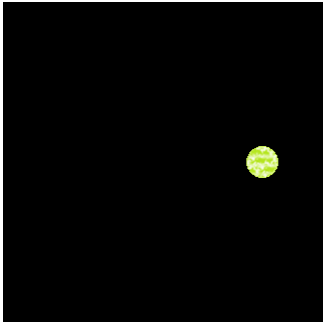
\includegraphics[scale=1]{frontend/prototype-0.png}
	\centering
	\caption{Erster Prototyp}
	\label{figx}
\end{figure}
\newpage
\section{Analyse - Steuerung}
\begin{quote}
	\href{https://github.com/Transport-Protocol/MBC-Ping-Pong/issues/11}{Analyse - Steuerung \#11}
	\newline
	\textit{Die Steuerung des Spiels erfolgt über das Handydisplay. Jedes Handy ist unterschiedlich groß, zudem sollte der Schläger nicht springen können.}
\end{quote}
Es zu analysieren wie sich verschiedene Auflösungen und verschiedene Pixeldichten auf das Spielgefühl auswirken können.
Denkbar ist das Geräte mit einer geringen Pixeldichte gegenüber Spielern mit einer hohen Pixeldichte im Vorteil sind da aus Geräten mit einer hohen Pixeldichte sehr viel kleinere Gesten zur Steuerung ausreichen.
\newline
\textbf{Zielsetzung dieser Analyse}
\begin{enumerate}
	\item
	      \textbf{Feststellung} Es soll festgestellt werden in wie weit sich ein Unterschied der Pixeldichte auf die Spielweise auswirken kann.
	\item
	      \textbf{Behandlung} Es soll geprüft werden ob sich eine mögliche Unfairness beheben lässt und ein mögliches Konzept erstellt werden.
\end{enumerate}
\subsection{Feststellung der Auswirkung verschiedener Pixeldichten}
Je nachdem wie die Steuerung implementiert wird die Pixeldichte eines Steuergerätes mehr oder weniger Einfluss auf das Spiel haben. Das birgt die Gefahr das Spieler mit einem Gerät mit einer geringen Pixeldichte gegenüber einem Spieler mit einem Gerät mit hoher Pixeldichte im Nachteil ist da er wesentlich stärkere Bewegungen auf der Touchfläche ausführen muss.
Theoretisch kann dies dazu führen das Spieler auf einem Tablet mit niedriger Auflösung immer im Nachteil zu Hochauflösenden Smartphones sind.
Laut der Android Spezifikation muss die Pixeldichte von Android Geräten mindestens 100 dpi betragen. Ferner sind in den Spezifikationen Pixeldichten bis zu 640dpi (xxxhdpi) definiert. Geräte mit 640dpi wären Geräten mit 100dpi um 640\% überlegen.
\paragraph{} Angenommen die Schläger würden 1:1 um den Pixelabstand der Controller bewegt werden und das Spielfeld habe eine Höhe von 400 Pixeln.
Auf einem Gerät mit 100dpi müsste der Spieler über eine Stecke von 4 cm streichen müssen um den Schläger von einem Ende zum anderen zu bewegen. Auf einem Gerät mit 640dpi müsste der Spieler nur über eine Stecke von unter einem Zentimeter streichen.
\subsection{Behandeln verschiedener Pixeldichten}
\paragraph{Ermitteln von der DPI im Browser}
\mbox{}\\
Es wird nach vorhanden Lösungen zum erkennen der Pixeldichte in PPI bzw DPI gesucht.
Die gefundenen Beispiele werden dann mit verschiedenen Geräten getestet und die Ergebnisse mit den tatsächlichen DPI verglichen.
\newline\textbf{Die Testgeräte}
\begin{enumerate}
	\item \begin{tabular}{cc}
	      Name & PC Monitor\\
	      Diagonale & 23.6zoll\\
	      Auflösung & 1920*1080\\
	      Pixeldichte & 93 DPI\\
	\end{tabular}
	\item \begin{tabular}{cc}
	      Name & Samsung Galaxy S4\\
	      Diagonale & 4.99zoll\\
	      Auflösung & 1920*1080\\
	      Pixeldichte & 441 DPI\\
	\end{tabular}
	\item \begin{tabular}{cc}
	      Name & Samsung Galaxy Tab A\\
	      Diagonale & 9.7zoll\\
	      Auflösung & 1024*768\\
	      Pixeldichte & 132 DPI\\
	\end{tabular}
\end{enumerate}
\newpage
\begin{itemize}
	\item
	      \textbf{http://www.infobyip.com/detectmonitordpi.php} Eine Website zur Ermittlung der DPI. Es wird ein Quadrat per CSS auf eine bestimmte Größe, zum Beispiel 1 Zoll, formatiert und dann die Größe in Pixeln ausgelesen. Auf diese Weise lässt sich ein DPI wert berechnen.
	      \newline
	      Tests:
	      %\begin{enumerate}
	      \begin{tabular}{ccc}
	      	                     & Erwarteter Wert & Ermittelter Wert           \\
	      	PC Monitor 1         &                 &                            \\
	      	Pixeldichte          & 93 DPI          & \colorbox{red!30}{96 DPI}  \\
	      	Größe des Feldes     & 8 cm            & \colorbox{red!30}{8.2 cm}  \\
	      	                     &                 &                            \\
	      	Samsung Galaxy S4    &                 &                            \\
	      	Pixeldichte          & 441 DPI         & \colorbox{red!30}{288 DPI} \\
	      	Größe des Feldes     & 8 cm            & \colorbox{red!30}{1.8 cm}  \\
	      	                     &                 &                            \\
	      	Samsung Galaxy Tab A &                 &                            \\
	      	Pixeldichte          & 132 DPI         & \colorbox{red!30}{96 DPI}  \\
	      	Größe des Feldes     & 8 cm            & \colorbox{red!30}{5.7 cm}  \\
	      \end{tabular}
	      %\end{enumerate}
	      Getestet wurde jeweils mit Firefox \& Chrome, der PC Monitor wurde auch noch mit dem Edge Browser getestet. Die Ergebnisse waren allesamt für das Gerät identisch.
	      \newline
	      \textbf{Ergebnis:} Die DPI wurden nicht korrekt erkannt. Die Werte weichen auf dem Mobiltelefon um bis zu \underline{77.5\%} ab.
\end{itemize}
\newpage
\paragraph{Verwenden von 'window.devicePixelRatio'}
\mbox{}\\
Die Eigenschaft \textit{window.devicePixelRatio} gibt das Verhältnis der Größe der physikalischen Pixel des aktuellen Displays zu der Größe der Geräteunabhängigen-Pixel (\textit{device independent pixels(dips)}) wieder.
\begin{displaymath}
	window.devicePixelRatio = physical pixels / dips 
\end{displaymath}

Es wird vor allem dafür genutzt um eine Einheitliche Darstellung von Webinhalten auf verschiedenen Displaygrößen zu erreichen.
\newline
Die Methode klingt sehr vielversprechend, also entschied ich einen Test zu erstellen. Meine Idee ist es ein Quadrat zeichnen zu lassen bei dem die Größe abhängig von dem devicePixelRatio ist und dann die Seitenlänge auf dem Display zu messen.
Mein verwendeter Code:
\begin{lstlisting}
var c=document.getElementById("myCanvas");
var ctx=c.getContext("2d");
var w = 100*window.devicePixelRatio;
ctx.rect(20,20,w,w);
ctx.fillText(w,30,30); 
ctx.stroke(); 
\end{lstlisting}

\textbf{Tests:}
\newline
\begin{tabular}{ccc}
	Gerät                  & DevicePixelRatio & Größe TestQuadrat   \\
	PC Monitor 23.6"       & 1.0              & 2.7 cm              \\
	Samsung Galaxy S4      & 3.0              & 1.9 cm              \\
	Samsung Galaxy Tab A   & 1.0              & 1.5 cm              \\
	Samsung Galaxy S3 Neo  & 2.0              & 1.3 cm              \\
	Samsung Galaxy S5 mini & 2.0              & 1.1 cm              \\
	Samsung Galaxy S7 edge & 4.0              & >4 cm               \\
\end{tabular}
\paragraph{Ergebnis:}
\mbox{}\\
Das Ergebnis der Tests ist leider ernüchternd. Die ersten Geräte zeigten das Quardrat allesamt in einer ähnlichen Größe. Doch auf weiteren Testgeräten zeigte sich das die Größe sehr stark variierte. Auf dem Samsung Galaxy S7 edge war das Quadrat sogar sehr viel größer als der vordefinierte Bereich.
\newpage
\paragraph{Suche nach Alternativen zu DevicePixelRatio}
\mbox{}\\
An vielen Stellen habe ich gelesen das der DevicePixelRatio sehr häufig gerundet wird. Dies fiel ebenfalls bei den Testgeräten auf.
\newline
Also kam mir die Idee eine eigene Version der Funktion zu schreiben. In Javascript kann man mit folgender Funktion testen ob ein bestimmter DevicePixelRatio unterstützt wird.
\begin{lstlisting}
if (window.matchMedia('(-webkit-min-device-pixel-ratio: 1)').matches) 
\end{lstlisting}
Meine Idee war es den gewünschten Wert der Funktion schrittweise zu erhöhen und den zuletzt akzeptierten Wert zurückzugeben.
\newline
Daraus ergab sich folgende Funktion:
\begin{lstlisting}
function getDPR() {
    var numb = 1.0;
    while(window.matchMedia(
    	'(-webkit-min-device-pixel-ratio: ' + numb + ')'
    	).matches) {
        	numb += 0.1;
    }
    return numb - 0.1;
}
\end{lstlisting}
Leider ergaben die Test mit dieser Funktion keine nennenswerte Ergebnisse weswegen ich auf eine Auflistung und Auswertung der Ergebnisse in diesem Falle verzichte.
\paragraph{Verwendung der CSS3 MediaQuery Eigenschaften}
\mbox{}\\
Mit CSS3 lassen sich verschiedene Fälle für verschiedene Auflösungen definieren.
\begin{figure}[ht]
	\centering
	\begin{lstlisting}
@media (resolution: 96dpi) { /* Exakt 96 Bildpunkte pro Zoll */ }
@media (min-resolution: 200dpcm) { /* Mindestens 200 Punkte pro cm */ }
@media (max-resolution: 300dpi) { /* Maximal 300 Punkte pro Zoll */ }
	\end{lstlisting}
	\caption{Quelle: https:\/\/wiki.selfhtml.org\/wiki\/CSS\/Media\_Queries}
	\label{figx}
\end{figure}
\newline
Hiermit ist es möglich für die verschiedenen Pixeldichten die Kontrollfelder anzupassen. Allerdings werden die Pixeldichten der Geräte nicht immer richtig erkannt. Es 
\newpage
\subsection{Ergebnis der Analyse}
Es gibt leider keine Möglichkeit eine Webapp mit exakten physikalischen Größen zu gestalten.
\paragraph{Gestaltung per CSS Einheiten} In CSS besteht die Möglichkeit Größen in CM oder Zoll zu definieren. Leider entsprechen die Werte auf Mobilen Endgeräten nicht den gewünschten Werten.
\paragraph{Gestaltung mit Device Pixel Ratio} Die Gestaltung per DevicePixelRatio erscheint wesentlich genauer als die Gestaltung mit CSS Längenangaben allerdings ist auch diese Lösung sehr ungenau und lässt sich nicht einheitlich nutzen. 
\paragraph{Gestaltung der Steuerung} Man könnte die Steuerung so definieren das ein Vorteil der Pixeldichte sich nicht zu sehr auf das Spiel auswirkt. Beispielsweise Kann man eine Maximalgeschwindigkeit der Schläger so definieren das sie auch auf Geräten mit geringer Pixeldichte leicht erreicht werden kann. Dadurch sind allerdings möglicherweise Geräte mit hoher Pixeldichte im Nachteil da man für kurze Bewegungen nur noch minimale Bewegungen auf dem Bildschirm durchführen dürfte.
\newline
Denkbar wäre auch eine Steuerung mit fester Bewegungsgeschwindigkeit sodass nur noch die Richtung der Schläger durch die Controller geregelt wird. Diese Art Steuerung verspricht allerdings nicht viel Spaß oder Reaktionsmöglichkeiten der Spieler.
\newline
\newline
\textbf{Lösungsmöglichkeit:}
\paragraph{Verrechnung der Information zur Pixeldichte} 
\mbox{}\\
Mit den CSS3 Media Queries ist es zumindest ansatzweise Möglich die Pixeldichte der Geräte zu erkennen. Allerdings sich auch sie sehr ungenau und keinesfalls verlässlich.
\newline
Zur fairen Gestaltung der Touchfelder sollten wir die Media Queries bzw den DevicePixelRatio verwenden um zwischen Geräten mit hoher und geringerer Pixeldichte unterscheiden.
\newline
Beispielsweise indem wir den PixelRatio mit der zurückgelegten Stecke in Pixeln verrechnen.
\begin{lstlisting}
movement = screenDistance / window.devicePixelRatio;
\end{lstlisting}
Somit werden Geräte mit einem PixelRatio von 1 nicht benachteiligt. Außerdem hat dies zur Folge das Spieler auf einem Gerät mit einem hohen PixelRatio ihre Schläger nicht unnötig schnell bewegen wenn sie zum Beispiel nur kurze Bewegungen erreichen wollen.
\newline 
Ein Problem bleibt jedoch, der PixelRatio ist nicht sehr genau. Um ein Gefühl für die Auswirkungen zu bekommen müssen wir mehrere Testgeräte für die Steuerung verwenden.
\subsection{Flüssige Bewegung}
Um eine flüssige Bewegung zu garantieren sollten wir uns auf einige Eigenschaften der Steuerung festlegen.
\paragraph{Anforderung: Bildschirmposition != Schlägerposition}
\mbox{}\\
Die Schläger sollen in Abhängigkeit einer Bewegung, also einer Positionsänderung auf dem Bildschirm bewegt werden. Das bedeutet für uns das wir die Information der Controller nicht als Absolute Positionen sehen sondern eher die Änderung während einer Geste betrachten.
\newline
Hierfür sei folgendes Festgelegt:
\begin{itemize}
	\item 
	      \textbf{Beginn der Geste:} Eine Geste beginnt mit dem Berühren des Touchfeldes. Die Startposition wird ermittelt und in einer Variable gespeichert.
	\item
	      \textbf{Während der Geste:} Während der Finger sich auf dem Touchfeld bewegt wird die neue Position des Fingers ausgewertet. Die neue Position wird von der alten Position abgezogen wodurch sich eine Differenz ergibt. Diese wird dann mit dem PixelRatio verrechnet und an das Spiel (DisplayPeer) geschickt.
	      \newline
	      Der ganze Prozess sollte alle 40ms neu gestartet werden.
	\item
	      \textbf{Ende einer Geste: } Eine Geste endet sobald das Touchfeld nicht mehr berührt wird. Die aktuelle Änderung der position wird auf 0 gesetzt.
\end{itemize}
Wenn der Controller nicht mehr berührt wird so darf sich der Schläger nicht weiter bewegen. Der Controller braucht in diesem Zustand dem Spiel keine Infos übermitteln.
\newline
Moderne Mobiltelefone haben wesentlich höhere Auflösungen als unser Spielfeld groß sein wird. Aus diesem Grund sollte die Bewegung auf einem Maximumwert begrenzt werden.
\newline 
Maximal sollte sich ein Schläger über die gesamte Spielfläche in einem Zyklus bewegen können. Es ist denkbar das wir den Wert später nach unten korrigieren müssen um ein gutes Spielgefühl schaffen zu können.

See also \cite{sample_bib}.


%%%%

%% appendix if used
%%\appendix
%%\typeout{===== File: appendix}
%%\include{appendix}

% bibliography and other stuff
\backmatter

\typeout{===== Section: literature}
%% read the documentation for customizing the style
\bibliographystyle{dinat}
\bibliography{MBC-Ping-Pong}

\typeout{===== Section: nomenclature}
%% uncomment if a TOC entry is needed
%%\addcontentsline{toc}{chapter}{Glossar}
\renewcommand{\nomname}{Glossar}
\clearpage
\markboth{\nomname}{\nomname} %% see nomencl doc, page 9, section 4.1
\printnomenclature

%% index
\typeout{===== Section: index}
\printindex

\HAWasurency

\end{document}
